\documentclass[12pt, openany, oneside, a4paper, english, brazil]{abntex2}   % Padrão Abntex2

%***************************** PACOTES *********************************** %
\usepackage[pdftex]{color,graphicx}

%\usepackage[within=none]{newfloat}
\usepackage[utf8]{inputenc}		     % Codificacao do documento (conversão automática dos acentos)


%	Fonte
\usepackage[T1]{fontenc}		   	 % Selecao de codigos de fonte.
\usepackage[brazil]{babel}
\usepackage{lmodern}			     % Usa a fonte Latin Modern

%	Matemático e Gráfico
\usepackage{float}
\usepackage{graphics,graphicx}	     % pacotes para inserir figuras .eps ou .jpg
\graphicspath{{figuras/}}            % pasta de figuras
\usepackage{amssymb}           		 % pacote para fontes e simbolos matemáticos
\usepackage{longtable}          	 % possibilita inserir grandes tabelas
\usepackage{makecell}                % possibilita pular linhas nas tabelas
\usepackage{xcolor,colortbl,multirow} % permite textos e tabelas com cores
\usepackage{amsmath}           		 % pacote para equações
\usepackage{epstopdf}
\usepackage{ragged2e}
\usepackage{listings}
%\lstset{numbers=left, numberstyle=\tiny, stepnumber=1, numbersep=5pt, basicstyle=\scriptsize ,frame=tbrl}
\usepackage{etoolbox}
\usepackage{multicol}
%\usepackage{caption}
\usepackage[position=b,singlelinecheck=on]{subfig}

\floatstyle{plaintop}
\newfloat{quadro}{htbp}{loq}
\floatname{quadro}{Quadro}

\makeatletter
\patchcmd{\listof}% <cmd>
{\float@listhead}% <search>
{\@namedef{l@#1}{\l@table}\float@listhead}% <replace>
{}{}% <success><failure>
\makeatother

%\makeatletter
%\renewcommand*{\float@listhead}[1]{%
%	\@ifundefined{chapter}{%
%		\section*{#1}%
%		\addcontentsline{toc}{section}{#1}%
%	}{%
%	\chapter*{#1}% 
%	\addcontentsline{toc}{chapter}{#1}%
%}%
%\@mkboth{\MakeUppercase{#1}}{\MakeUppercase{#1}}%
%}
%\makeatother




%\DeclareFloatingEnvironment{quadro}[Quadro][Lista de quadros]
%\DeclareCaptionType{quadro}[Quadros][Lista de quadros]


% % % % % % % % % % % % % % % % % % % %

\definecolor{codegreen}{rgb}{0,0.6,0}
\definecolor{codegray}{rgb}{0.5,0.5,0.5}
\definecolor{codepurple}{rgb}{0.58,0,0.82}
\definecolor{backcolour}{rgb}{0.95,0.95,0.92}

%\definecolor{verde}{rgb}{0,0,0}

\lstdefinestyle{mystyle}{
	backgroundcolor=\color{backcolour},   
	commentstyle=\color{codegreen},
	keywordstyle=\color{magenta},
	numberstyle=\tiny\color{codegray},
	stringstyle=\color{codepurple},
	basicstyle=\footnotesize,
	breakatwhitespace=false,         
	breaklines=true,                 
	captionpos=b,                    
	keepspaces=true,                 
	numbers=left,                    
	numbersep=5pt,                  
	showspaces=false,                
	showstringspaces=false,
	showtabs=false,                  
	tabsize=2
}

\lstset{style=mystyle}

%	Estrutural
\usepackage{url}
\usepackage{threeparttable}     	 % permite a inserção de notas de rodapé nas tabelas
\usepackage{lscape}             	 % orientação de página LANDSCAPE
\usepackage{pifont}             	 % acrescenta símbolos diferentes.
%\usepackage{cmap}					 % Mapear caracteres especiais no PDF	
\usepackage{lastpage}				 % Usado pela Ficha catalográfica
\usepackage{indentfirst}			 % Indenta o primeiro parágrafo de cada sessão.



% Pacotes de citações
\usepackage[brazilian,hyperpageref]{backref}	 % Paginas com as citações na bibl
\usepackage[alf]{abntex2cite}	% Citações padrão ABNT numerica
     
% remover bordas dos links
\hypersetup{
    colorlinks,
    linkcolor={black},
    citecolor={black},
    urlcolor={black}
} % resto dos pacotes Latex
%\usepackage[english]{style/UCSAL-Template} % personalização da ABNTEX2 para escrita em inglês
\usepackage[portuguese]{style/ucsal} % personalização da ABNTEX2 para escrita em português
\usepackage{longtable}
\usepackage{blindtext}
\DisemulatePackage{setspace}
\usepackage{setspace}
\usepackage{lipsum}
\usepackage[left=3cm,top=3cm,right=2cm,bottom=2cm]{geometry}
\usepackage{fontspec}
\setmainfont{Arial}
\usepackage{hyperref}
\usepackage{graphicx}
\usepackage{caption}
\usepackage{subcaption}





%inserindo apenas uma página

%---------------------------------------------------------------
%--------- DADOS BÁSICOS DO TRABALHO (Preencher todos) ---------
%---------------------------------------------------------------


\titulo{A GAMIFICAÇÃO COMO ESTRATÉGIA PARA O ENSINO DE MATEMÁTICA BÁSICA PARA ALUNOS DO ENSINO FUNDAMENTAL I
}   % Título do Trabalho em Português

\tituloingles{GAMIFICATION AS A STRATEGY FOR BASIC MATHEMATICS TEACHING FOR ELEMENTARY SCHOOL I STUDENTS}   % Título do Trabalho em Inglês

\palavraschave{1. Gamificação.
2. Educação Matemática.
3. Aplicativo educacional.}  % 5 palavras-chave

\keywords{1. Gamification.
2. Mathematics Education.
3. Educational App.}   % 5 palavras-chave para resumo em inglês

\DEELautor{ Cristiano da Silva Oliveira Filho\\Enzo Santana de Almeida\\ Jamile Santos Da Conceição\\ Lucas Augusto Assunção Garcia Walter  \\Vinicius dos Santos Candeias\\}{} % Alunos autores do trabalho



\curso{Bacharelado em Engenharia de Software}												
\orientador{Andre Ricardo Magalhães}  % Professor Orientador membro da banca 

\membrob{Prof. Me. Segundo professor}   % Professor membro da banca 
\membroc{Prof. Me. Terceiro professor}   % Professor membro da banca

\local{Salvador}   % Cidade da instituição
\data{2024}        % Ano de realização

%--------------------------------------------------------------------------------------------



\begin{document}
\onehalfspacing

% Seleção automática do idioma, não alterar
\ifx\isenglish\undefined
    \selectlanguage{brazil}
\else
    \selectlanguage{english}
\fi

% Texto da Dedicatória (OBS: dedicatória é opcional)
% Caso não queira inserir, deixe em branco ( \dedicatoria{} )
\DEELdedicatoria{Dedico este trabalho a todos aqueles.... \\}  
    
% Texto dos Agradecimentos (OBS: Agradecimentos é opcional)
% Caso não queira inserir, deixe em branco ( \agradecimentos{} )
\DEELagradecimentos{Eu Cristiano agradeço primeiramente a Jeová Deus e a minha família que sempre me apoiou nessa trajetória com todas as adversidades.} 

                       
% Texto da Epígrafe (OBS: Epígrafe é opcional)
% Caso não queira inserir, deixe em branco ( \epigrafe{} )
\DEELepigrafe{\textit{"A alegria está na luta, na tentativa, no sofrimento envolvido e não na vitória propriamente dita."} \\ (Mahatma Gandhi 
)} 
    

% Texto do Resumo (OBS: Resumo é Obrigatório)
\DEELresumo{
Em atendimento ao Trabalho de Conclusão de Curso; A GAMIFICAÇÃO COMO ESTRATÉGIA PARA O ENSINO DE MATEMÁTICA BÁSICA PARA ALUNOS DO ENSINO FUNDAMENTAL I, apresentado à Universidade Católica do Salvador como parte dos requisitos necessários para a obtenção do Título de Engenheiro de Software sob a Orientação e docência de André Ricardo Magalhães. O presente trabalho tem como objetivo evidenciar a importância da diretriz e aplicação do ensino da matemática através de novas praticas docente, buscando contribuir com ênfase nos conteúdos, mediante o uso de softwares específicos (aplicativos de jogos educacionais) com a utilização de metodologias ativas que são estratégias de ensinamento que incentivam os estudantes a aprenderem de forma autónoma e participativa, por intervenção da gamificação no Ensino Fundamental I, almejando auxiliar, visando conseguir solucionar um problema que tem se transformado em um grande desafio, onde os alunos frequentemente demonstram maior dificuldade nessa área. Para nortear esse estudo foram utilizados, como referência, os seguintes autores: Creswell (2013), Furlan (2016), Nóvoa (2004), Almeida (2008), Josso (1988, 2004), Bueno (1996), Lima (2008), Passegi (2003), Pimenta e Lima ( 2004), Pineau (1988), Souza (2004), Kleiman (2005), Freire (2003), Soares (2004), Moran (2006), Molica (2009) e Street (2014) além de outros. Constata-se que a complexidade para encontrar um equilíbrio na instrução desta disciplina com métodos convencionais permeiam os ambientes escolares. Uma pesquisa internacional feita por um site de tecnologia, mostrou que brasileiros lideram em tempo de uso de telas de celulares e outros dispositivos eletrónicos. Cerca de nove horas e meia utilizando esses aparelhos, demonstrando um alto nível de conectividade digital no país. Concluiu-se a necessidade de promover atividades que utilizem as ferramentas de tecnologias digitais, softwares e determinados aplicativos como um auxilio favorável a educação.} 
     
% Texto do Abstract (OBS: Abstract é Obrigatório)
\DEELabstract{
In compliance with the Course Completion Work; GAMIFICATION AS A STRATEGY FOR THE TEACHING OF BASIC MATHEMATICS FOR ELEMENTARY SCHOOL I STUDENTS presented to the Catholic University of Salvador as part of the requirements for obtaining the Title of Software Engineer under the guidance and teaching of André Ricardo Magalhães. The present work aims to highlight the importance of the guideline and application of mathematics teaching through new teaching practices, seeking to contribute with emphasis on content, through the use of specific software (educational games applications) with the use of active methodologies that are teaching strategies that encourage students to learn autonomously and participatively, through the intervention of gamification in Elementary School I, aiming to solve a problem that has become a great challenge, where students often show greater difficulty in this area. To guide this study, the following authors were used as reference: Creswell (2013), Furlan (2016), Nóvoa (2004), Almeida (2008), Josso (1988, 2004), Bueno (1996), Lima (2008), Passegi (2003), Pimenta e Lima ( 2004), Pineau (1988), Souza (2004), Kleiman (2004) (2003), Soares (2004), Moran (2006), Molica (2009) and Street (2014) among others. It appears that the complexity to find a balance in the instruction of this discipline with conventional methods permeate the school environments. An international survey by a technology site showed that Brazilians lead in time to use mobile screens and other electronic devices. About nine and a half hours using these devices, demonstrating a high level of digital connectivity in the country. It was concluded the need to promote activities that use the tools of digital technologies, software and certain applications as a favorable aid to education.
} 
    



%%%%%%%%%%%%%%%%%%%%%%%%%%%
%% Elementos Pré-Textuais%%
%%%%%%%%%%%%%%%%%%%%%%%%%%%
\ElementosPreTextuais
% Insere todos os elementos Pré-Textuais listados (capa, folha de rosto, ...)
    % capa                   % Obrigatório
    % folhaderosto           % Obrigatório
    % folhaaprovacao         % Obrigatório
	% dedicatoria            % Opcional
	% agradecimentos         % Opcional
    % epigrafe               % Opcional
    % resumo                 % Obrigatório
    % abstract               % Obrigatório

%\newpage
%--------Lista de figuras--------
\ListaDeFiguras 
%--------Lista de tabelas--------
\ListaDeTabelas 
%--------Lista de Siglas e Abreviaturas--------
%----------Lista de Acronimos --------------------------------
\ifx\isenglish\undefined
\pretextualchapter{Lista de Siglas e Abreviaturas}
\else
\pretextualchapter{Acronyms}
\fi


%\renewcommand{\baselinestretch}{2} %espaçamento entre linhas (por definicçào, no espABNT é 2)
\begin{tabbing}
xxxxxxxxxxx \= xxxxxxxxxxxxx \kill
\textsc{API}            \> \textit{Application Programming Interface}\\

\textsc{BES}            \> \textit{Bacharelado em Engenharia de Software}\\

\textsc{RF}             \> \textit{Requisitos Funcionais}\\

\textsc{RNF}            \> \textit{Requisitos Não Funcionais}\\

\textsc{RN}            \> \textit{Regra de Negócio}\\

\textsc{MVP}            \> \textit{Mínimo Produto Viável}


\end{tabbing}

%\addcontentsline{toc}{chapter}{Lista de Siglas e Abreviaturas}
   
%--------Lista de Simbolos e Notação--------
%\include{list_simbolos} 
%--------Sumário-------
\Sumario


%%%%%%%%%%%%%%%%%%%%%%
%%Elementos Textuais%%
%%%%%%%%%%%%%%%%%%%%%%
\textual 
\chapter{Introdução}\label{chp:intro}

Em síntese, refletir de forma lúdica e interativa, pode estabelecer uma conexão com os alunos interligados à matemática. Se fez necessário a criação de uma ideologia de  aplicação representado por um personagem chamado Polvo Pi, desenvolvido para conduzir e motivar principalmente o público infantil e interessados no aprendizado através da aplicação educativa. A missão principal do persona é ajudar o colegiado do Ensino Fundamental I, trazendo vínculos e identificações por parte dos estudantes, despertando a descobrirem como a matemática pode ser divertida e fascinante, utilizando jogos, desafios e histórias envolventes para ensinar conceitos matemáticos de maneira simples, conduzindo a imersão em um novo mundo numa troca constante de conhecimento. \cite{Lopes2020}

Math.Pow acredita que as dificuldades enfrentadas no ensino da matemática podem ser superadas com o auxílio da tecnologia como ferramenta, bastando encontrar a maneira certa de aprender. A aplicação tem como principal objetivo viabilizar a elaboração de metodologias de ensino através de planejamentos pedagógicos eficientes e criativos. A escolha do melhor nome para representar essa nova ferramenta, está coerente a fatores científicos, relações e comparações. Sendo assim o nome escolhido é “Math.Pow”:

POLVO: é um animal marinho de corpo mole e flexível, possuindo oito braços chamados tentáculos, conhecido por sua inteligência, habilidades de camuflagem e comportamentos complexos; ele serve como inspiração para a idealização da aplicação educativa. Da família dos cefalópodes, este molusco busca se adaptar a uma variedade de ambientes para sobreviver. Por analogia, sob o mesmo ponto de vista. Do mesmo modo, a ideia em forma de aplicação se adapta às diferentes maneiras de aprendizado dos alunos, utilizando as características-chave desse fascinante mamífero pelágico almejando tornar o ensino mais eficaz e envolvente.\cite{BBC2023}




\section{Aplicabilidade e Motivação}\label{chp:aplic}

A dificuldade encontrada na docência do Ensino Fundamental I nas atribuições das aulas de matemática, tratam-se de abordagens que proporcionam alternâncias e intercorrências consideráveis. Os problemas, contratempos e adversidades apresentam-se desde os planejamentos pedagógicos por coordenadores em planos de cursos e sobrevêm chegando até os docentes em seus planos de aulas que não conseguem atingir com eficiência o entendimento e absorção da aprendizagem pelos discentes. 

Tanto o magistério quanto o alunato enfrentam objeções ao lidar com essa disciplina, procurando superar muitos obstáculos, ponderando que os incentivos deparam em grande parte dos estudantes que não consideram a matemática como algo notável ou concebível em suas vivências. Além disso, os estímulos para aprendizagem, aplicação das suas concepções e ideias são diretamente impactados. Igualmente a subjetividade e complexidão da matemática abrange concepções subjetivas e constantemente abstrusa, existindo a possibilidade do alunado encontrar obstruções para perceber e assimilar os conceitos, o que pode trazer o desapontamento. 

Da mesma forma a fixação e cognição dos estudantes focalizam em memorar os métodos e suas fórmulas em vez de tentar compreender os princípios implícitos subentendidos, impossibilitando a sua criatividade para solucionar determinadas questões com eficacia. Assim também as ferramentas necessárias para os educadores deparam-se com impedimentos para obter materiais instrutivos, compatíveis e metodologias de transmissão de conhecimentos eficientes, considerando a probabilidade de impactos negativos na natureza da orientação. Por analogia a aflição pela disciplina é perceptível em grande parte dos alunos que se apresentam ansiosos, pois o processo de aprender matemática oferece tendências que afetam a conduta e autoestima. 

Atualmente a maior parte dos jovens e até mesmo alguns adultos vivenciam a sensação de experienciar jogos com parâmetros físicos ou digitais por intermédio de videogames, computadores, smartphones, dominós, baralhos, dados etc. Subsiste neles alguma coisa indeterminada que atrai e magnetiza, tomando por completo a atenção do usuário. Que idealiza a sobrelevação, individualmente ou em equipe, incentivado com o resultado alcançado em suas fases, etapas, níveis e etc. Pois mesmo parecendo uma simples diversão, nas variadas formas e possibilidades de jogos se aplica energia espontaneamente. Além disso as atividades de entretenimentos, define a estruturação intrínseca mediante a diretrizes que tem por objetivo conduzir a atividade com procedimentos organizados.

\section{Contextualização}

A gamificação, que utiliza elementos de jogos para engajar e motivar os alunos, tem se destacado como uma abordagem eficaz para o ensino. A gamificação oferece oportunidades de aprendizado interativo, onde desafios, recompensas e feedbacks imediatos podem tornar a experiência educacional mais estimulante e atraente para as crianças.

A evolução das tecnologias tem facilitado significativamente a inclusão de pessoas com deficiência, proporcionando maior acessibilidade e autonomia. Novos recursos e APIs que facilitam a interconexão e integração entre plataformas, têm possibilitado o desenvolvimento de aplicações e soluções tecnológicas que atendam a um número cada vez maior de usuários com necessidades especiais. Um exemplo disso é o aplicativo "Hand Talk", que disponibiliza um plugin para integrações de acessibilidade a deficientes auditivos, permitindo tradução automática para Língua Brasileira de Sinais.

Outras iniciativas importantes são ferramentas de leitura de tela, ampliação de conteúdo, contraste elevado e interfaces adaptáveis. Essas inovações têm o poder de reduzir barreiras, promover inclusão digital e transformar positivamente a vida de pessoas com deficiência. Como destaca  \cite{furlan2016desenvolvimento}, "a tecnologia tem um papel crucial na promoção da acessibilidade e inclusão das pessoas com deficiência".


\section{Objetivos}

Afinal de contas, qual é a definição de gamificação? Quais são os pontos de uniformidade, divergência e convergência entre gamificação e jogos? Como pôr em prática? Neste estudo acadêmico, a abordagem da gamificação será abrangente, com reflexões e idealizações que se referem a um tema atual que estabelece relações de grande importância no âmbito da educação.O elemento conceitual investigativo deste objeto de pesquisa é muito significativo, dado que a gamificação requer um entendimento satisfatório para ser empregue com eficiência, sensatez e seriedade. A temática será abordada em tópicos considerados relevantes. Investigando as concepções e ideias empregadas, os recursos e componentes adotados, referenciando determinadas finalidades. Destarte, busca-se obter um entendimento referente ao conteúdo discutido neste trabalho de pesquisa e investigação científica, considerando que esta abordagem dissertada se trata de uma esfera que denota grande relevância mostrando considerável importância no campo acadêmico.


\subsection{Objetivo Geral}

 O principal objetivo desse trabalho de conclusão de curso é analisar o uso da gamificação através de um aplicativo,  enquanto uma metodologia ativa , para o ensino de matemática, com  alunos do fundamental I. Como ferramenta para auxílio na pesquisa temos como objetivo inicial a produção um aplicativo que usa elementos de gamificação, a escolha de um aplicativo é que não tenha a necessidade de ser usado somente em sala de aula, e sim para servir como ferramenta auxiliar no processo de ensino.


\subsection{Objetivos Específicos}

\begin{itemize}
\item{Autenticar se o uso de jogos educacionais para o ensino de matemática é eficaz.
}
\item {Avaliar quais conteúdos são mais estruturantes para o ensino da matemática no fundamental I.
} 
\item {Desenvolver sequências didáticas com a metodologia da gamificação.
 }  
\item {Desenvolver um aplicativo com uso das técnicas de gamificação.
}
\item {Validar o uso do aplicativo com professores e estudantes.
}
\item {Auxiliar no ensino de matemática para alunos do ensino fundamental I.
}
\end{itemize}

\section{Estrutura do Trabalho}

No Capítulo 1 é apresentado o objetivo geral e objetivos específicos, enquanto que o Capítulo 2 traz a Fundamentação Teórica. No Capítulo 3 está apresentada a metodologia do trabalho, enquanto que no Capítulo 4 são apresentados o experimento e coleta de dados. Finalmente, no Capítulo 5 é apresentada a conclusão desta monografia.


 % Texto do cap1.tex
\chapter{Fundamentação Teórica}\label{chp:rev}
\section{Ensino e Aprendizagem}

A aprendizagem é um processo que envolve a interação entre o professor e o aluno, sendo o papel do professor central para que o ensino seja eficaz. Conforme mencionado por \cite{DubetMartucelli1996}, o sistema escolar deve cumprir duas funções fundamentais: a construção de um indivíduo autônomo, capaz de refletir e se autorregular, e a socialização, que promove a integração de normas e valores sociais. Nesse sentido, a escola se torna um ambiente que perpetua a experiência humana como cultura, conforme destaca \cite{Forquin1992}.

A concepção construtivista, segundo \cite{Scheerens2004}, enfatiza a interdependência entre ensino e aprendizagem, tratando-os como processos inseparáveis. Nesse modelo, a aprendizagem é definida como “um processo de construção de significados e atribuição de sentido”, enquanto o ensino consiste na “ajuda necessária para que esse processo se realize na direção desejada”. Essa ajuda deve ser ajustada às necessidades e características do aluno, promovendo desafios acessíveis e que estimulem a reconstrução dos conhecimentos prévios, como argumentado por \cite{MarchesiMartin2003}.

Ainda sobre as práticas do professor, \cite{Onrubia1993}, citado em \cite{MarchesiMartin2003}, ressalta que a ajuda educativa só será eficaz se for capaz de mobilizar os esquemas de conhecimento do aluno e forçar sua reestruturação. Isso implica oferecer um ensino que se conecte diretamente à realidade e ao contexto dos estudantes, promovendo um aprendizado significativo.

O modelo QAIT, proposto por \cite{Slavin1986}, destaca que quatro elementos são essenciais para um ensino eficaz: qualidade da instrução, adequação ao nível dos alunos, incentivo à aprendizagem e tempo suficiente para absorção do conteúdo. Esses elementos devem estar integrados para garantir a eficácia do processo de ensino-aprendizagem.

Por outro lado, a perspectiva afetiva do professor também é essencial. Segundo \cite{FukudaPasquali2002}, aspectos como empatia, relacionamento positivo com os alunos e motivação são cruciais para estabelecer um ambiente de aprendizado efetivo. Esses elementos são complementados por características técnicas, como o domínio do conteúdo e a clareza na comunicação, conforme discutido por \cite{Silva1992}.

Em suma, a eficácia do ensino está diretamente relacionada à capacidade do professor de equilibrar habilidades técnicas e afetivas, adaptando suas estratégias às necessidades dos alunos e promovendo um ambiente de aprendizado inclusivo e motivador. Como destacam \cite{RosenshineStevens1986}, a interação entre práticas instrutivas bem planejadas e a adaptação ao ritmo dos estudantes é fundamental para garantir o sucesso educacional.

O ensino é um processo complexo que envolve tanto habilidades técnicas quanto interpessoais, sendo essencial para promover a aprendizagem e o desenvolvimento dos estudantes. Segundo \cite{DubetMartucelli1996}, o ensino eficaz deve desempenhar duas funções fundamentais: formar indivíduos autônomos, capazes de analisar e regular suas próprias ações, e promover a socialização, integrando normas, valores e conhecimentos que os preparem para participar ativamente na sociedade.

No contexto pedagógico, a eficácia do ensino depende de uma combinação de fatores. \cite{Scheerens2004} ressalta que o ensino deve ser entendido como um suporte contínuo para a construção de significados pelos alunos. Essa perspectiva destaca a importância da interação entre professor e aluno, considerando que a qualidade do ensino está diretamente relacionada à capacidade do professor de ajustar suas estratégias às necessidades de aprendizagem.

A prática pedagógica também se beneficia de modelos teóricos, como o modelo de ensino eficaz proposto por \cite{Slavin1986}. O modelo QAIT enfatiza quatro elementos essenciais: qualidade da instrução, adequação do nível de ensino, incentivo e tempo. Esses fatores, segundo o autor, precisam ser integrados e adaptados ao contexto para que o ensino produza os resultados esperados.

Além disso, a literatura destaca a importância de práticas pedagógicas baseadas em princípios reguladores. \cite{BrophyGood1986} argumentam que estratégias como o uso de reforços positivos, a interação ativa entre professor e alunos e a clareza na organização das aulas são fundamentais para a eficácia do ensino. Essas práticas, ao serem aplicadas, facilitam o aprendizado e promovem o desenvolvimento de habilidades cognitivas e emocionais.

Outro ponto relevante é o papel do professor na mediação do conhecimento. Conforme \cite{MarchesiMartin2003}, o professor eficaz não apenas transmite conteúdos, mas também ajuda os alunos a conectar novos conhecimentos com os já existentes. Essa abordagem reflete o ensino como um processo dinâmico e adaptativo, no qual o professor atua como facilitador da aprendizagem.

Por fim, \cite{RosenshineStevens1986} apontam que estratégias como a revisão do conteúdo, prática supervisionada e feedback contínuo são elementos chave para o ensino eficaz. Essas práticas permitem que os alunos consolidem o aprendizado de forma progressiva, garantindo a retenção e a aplicação prática dos conhecimentos adquiridos.

Em suma, o ensino eficaz é caracterizado por uma interação equilibrada entre planejamento, comunicação, motivação e adaptação às necessidades dos alunos. Essa abordagem, conforme os autores destacados, é essencial para promover o sucesso acadêmico e o desenvolvimento integral dos estudantes.

Entende-se que os métodos de ensino e de aprendizagem são expressões educacionais e, ao mesmo tempo, uma resposta pedagógica às necessidades de apropriação sistematizada do conhecimento científico em um dado momento histórico representando um processo dialético de produção \cite{lacanallo2007metodos}.

\section{Modelos de Ensino}
No processo de ensino-aprendizagem existem diferentes modelos de ensino que os professores podem utilizar para repassar o conteúdo da disciplina e a sua bagagem de conhecimento a respeito do assunto para os alunos \cite{kruger2013metodo}. Nesta seção, apresentamos um panorama dos principais modelos de ensino, explorando suas características e potencialidades, buscamos criar um contexto para a análise da gamificação, evidenciando como essa abordagem pode se integrar e complementar as práticas pedagógicas existentes, com o objetivo de tornar o aprendizado da matemática mais envolvente, significativo e eficaz para os alunos.

\subsection{Ensino Tradicional}

O ensino tradicional, enraizado na história da educação, é caracterizado pela centralização do professor como figura de autoridade e transmissor de conhecimento \cite{kruger2013metodo}. Segundo \cite{mezzari2011}, nessa abordagem o aluno assume um papel passivo, recebendo informações de forma estruturada e com ênfase na memorização de conteúdos . As aulas expositivas, nas quais o professor apresenta o conteúdo de forma oral, são uma das principais metodologias utilizadas nesse método \cite{weintraub2011}.

No ensino tradicional, o professor define o conteúdo programático, a organização das aulas e as atividades a serem realizadas pelos alunos \cite{santos2011}. A ênfase está na reprodução do conhecimento transmitido pelo professor, muitas vezes por meio de exercícios e atividades que visam a fixação do conteúdo \cite{pinho2010}.

Embora o método tradicional seja criticado por sua falta de flexibilidade e por não estimular a autonomia e o pensamento crítico dos alunos \cite{backes2010}, ele ainda é amplamente utilizado em diversos contextos educacionais \cite{teofilo2009}. Alguns autores defendem que o método tradicional pode ser eficaz em determinadas situações, como no ensino de conceitos básicos e na transmissão de informações de forma clara e concisa \cite{oliveira2012}. No entanto, a crítica predominante é que esse método não favorece o desenvolvimento de habilidades como a resolução de problemas, a criatividade e o pensamento crítico, que são cada vez mais importantes no mundo atual \cite{haddadetal1993}.

\subsection{Construtivismo}
O construtivismo, baseado nas teorias de Piaget e Vygotsky, é um método de ensino que coloca o aluno como protagonista no processo de aprendizagem \cite{coria-sabini2003,gomesbellini2009}. Nessa abordagem, o professor atua como facilitador, incentivando a construção do conhecimento por meio da interação do aluno com o ambiente e com os outros \cite{haddadetal1993}. O aluno é encorajado a descobrir o conteúdo por meio de pesquisas e atividades que promovam a reflexão e a compreensão \cite{coria-sabini2003}.

No método construtivista, o professor não é mais o detentor absoluto do conhecimento, mas sim um guia que auxilia o aluno a desenvolver suas próprias ideias e conclusões \cite{coria-sabini2003}. A ênfase está no aprendizado ativo, na experimentação e na resolução de problemas, buscando estimular a autonomia e o pensamento crítico dos alunos \cite{pinho2010}.

Uma das vantagens do método construtivista é a possibilidade de utilizar diversas fontes de informação, como livros, internet e outros recursos, para enriquecer o processo de aprendizagem \cite{chahuanjimenez2009}. Além disso, o trabalho em grupo é valorizado como forma de promover a colaboração, a troca de ideias e o desenvolvimento de habilidades sociais \cite{cogo2006}.

Apesar de suas potencialidades, o método construtivista também apresenta desafios, como a dificuldade do professor em conduzir uma turma com diferentes ritmos de aprendizagem e a necessidade de um planejamento cuidadoso das atividades para garantir que os alunos alcancem os objetivos de aprendizagem \cite{haddadetal1993,pinho2010}.

Dentro do modelo construtivista, diversas metodologias de ensino se destacam, como a Aprendizagem Baseada em Projetos, a Sala de Aula Invertida e a Gamificação, entre outras. Estas serão exploradas nas próximas seções.

\subsubsection{Aprendizagem Baseada em Projetos}

A Aprendizagem Baseada em Projetos (ABP) é uma metodologia ativa que se destaca por sua abordagem dinâmica e centrada no aluno \cite{alecia2022}. Em contraste com as metodologias tradicionais, nas quais o professor assume o papel central de transmissor de conhecimento, a ABP coloca o aluno como protagonista do processo de aprendizagem \cite{fartura2007}.

Na ABP, os alunos são desafiados a investigar e solucionar problemas reais e relevantes para o seu contexto, o que estimula o desenvolvimento de habilidades como pensamento crítico, colaboração, comunicação e autonomia \cite{moran2014}. Ao longo do projeto, os alunos se envolvem em atividades práticas, pesquisas, experimentos e discussões, construindo o conhecimento de forma ativa e significativa.

Um dos pontos fortes da ABP é a sua flexibilidade e adaptabilidade a diferentes áreas do conhecimento e níveis de ensino \cite{bacich2018}. No contexto do ensino de química, por exemplo, a ABP pode ser utilizada para explorar temas como sustentabilidade, meio ambiente, saúde e tecnologia, tornando o aprendizado mais relevante e conectado à realidade dos alunos.

Para que a ABP seja implementada com sucesso, é fundamental que os professores estejam preparados para assumir o papel de mediadores e facilitadores do processo de aprendizagem \cite{diesel2017}. Isso implica em planejar e estruturar o projeto de forma clara, definir objetivos de aprendizagem significativos, selecionar recursos adequados e acompanhar o progresso dos alunos de forma individualizada.

Em suma, a Aprendizagem Baseada em Projetos (ABP) representa uma abordagem pedagógica inovadora e promissora, capaz de transformar a forma como os alunos aprendem e se envolvem com o conhecimento \cite{arthur2020}. Ao adotar a ABP, os professores podem criar experiências de aprendizagem mais engajadoras, significativas e relevantes para os alunos, preparando-os para os desafios do século XXI.

\subsubsection{Sala de Aula Invertida}

A Sala de Aula Invertida (SAI) é uma metodologia ativa de ensino e aprendizagem que propõe uma inversão do modelo tradicional. O estudo do conteúdo conceitual, tipicamente realizado em sala de aula, passa a ser feito em casa pelo aluno, enquanto as atividades reflexivas e de resolução de dúvidas, geralmente feitas em casa, são transferidas para a sala de aula \cite{Bergmann_2016}.

\cite{Pavanelo_2017} diz que essa inversão tem como objetivo central tornar o aluno protagonista do seu processo de aprendizagem, incentivando a autonomia e a responsabilidade. Ao estudar o conteúdo previamente, o aluno chega à sala de aula com uma base de conhecimento, permitindo que o tempo em sala seja dedicado à discussão, resolução de dúvidas e atividades práticas, com o professor atuando como mediador e facilitador .

De acordo com \cite{Pavanelo_2017} a (SAI) se mostra particularmente relevante no contexto atual, em que as tecnologias digitais estão cada vez mais presentes na vida dos alunos. A flexibilidade de horários e a personalização do ensino, características dessa metodologia, atendem às necessidades dos estudantes que estão constantemente conectados ao mundo virtual .

Pesquisas indicam que a SAI pode ser aplicada com sucesso em diversas etapas da Educação Básica, desde os anos iniciais do Ensino Fundamental até o Ensino Médio, promovendo maior participação dos alunos e aprendizagem significativa \cite{Muraro_2019,Sanches_2019}.

Segundo \cite{Bergmann_2016} algumas das vantagens da SAI, incluem :
\begin{itemize}
\item Maior engajamento e responsabilidade do aluno no processo de aprendizagem 
\item Flexibilidade de tempo e personalização do ensino, atendendo às necessidades individuais dos alunos.
\item Otimização do tempo em sala de aula, permitindo que o professor se dedique mais às dúvidas e dificuldades dos alunos.
\item Possibilidade de revisão do conteúdo quantas vezes forem necessárias, com o aluno controlando o ritmo do aprendizado.
\item Fortalecimento da relação professor-aluno e aluno-aluno, por meio de atividades colaborativas e interação em sala de aula.    
\end{itemize}

No entanto, é importante ressaltar que a implementação da SAI exige planejamento e dedicação por parte do professor. A produção de materiais adequados, a escolha de plataformas online e a criação de estratégias para o tempo em sala de aula são alguns dos desafios a serem enfrentados \cite{Rodrigues_2020}.

\subsubsection{Gamificação}

A gamificação, segundo \cite{busarello2014gamificacao}, é a aplicação de elementos de jogos em contextos que não são jogos, como ambientes educacionais. Essa técnica visa aumentar o engajamento e a motivação dos alunos, utilizando elementos como competição, recompensas, desafios e feedbacks instantâneos . No contexto educacional, a gamificação pode tornar o aprendizado mais envolvente e atraente, estimulando a motivação dos estudantes e facilitando o engajamento com o conteúdo \cite{goncalves2021modelo}.

\cite{piaget1993formacao} destaca a importância do jogo no desenvolvimento infantil, argumentando que, ao jogar, a criança desenvolve suas percepções, inteligência e instintos sociais . A gamificação, ao incorporar elementos lúdicos no processo de ensino-aprendizagem, alinha-se com a visão de Piaget sobre a importância do jogo na educação.

\cite{vigotsky2007formacao} também contribui para a compreensão da gamificação na educação . Sua teoria sociocultural enfatiza a importância da interação social na aprendizagem, e a gamificação pode ser uma ferramenta poderosa para promover essa interação. Ao trabalhar em equipe, colaborar e competir em jogos educativos, os alunos desenvolvem habilidades sociais e cognitivas importantes.

A gamificação também se alinha com a teoria de \cite{keller2017development}, conhecida como ARCS (Atenção, Relevância, Confiança e Satisfação) . Essa teoria destaca os elementos necessários para motivar o aluno no processo de aprendizagem. A gamificação, ao utilizar elementos de jogos como desafios, recompensas e feedbacks, pode atender a esses elementos e aumentar a motivação e o engajamento dos alunos.

Outro conceito relevante é o de fluxo, discutido por \cite{hamari2014measuring}. O fluxo é um estado de concentração profunda e envolvimento em uma atividade desafiadora. A gamificação, ao criar atividades desafiadoras e recompensadoras, pode levar os alunos a experimentarem o estado de fluxo, aumentando sua concentração e engajamento no aprendizado.

Em suma, a gamificação é uma abordagem pedagógica que encontra respaldo em diversas teorias educacionais e psicológicas. Ao incorporar elementos de jogos no processo de ensino-aprendizagem, a gamificação pode aumentar a motivação, o engajamento e a participação dos alunos, tornando o aprendizado mais eficaz e significativo.

\section{Jogos}

Jogos, em suas diversas formas e manifestações, têm acompanhado a humanidade ao longo de sua história, servindo como ferramentas de entretenimento, socialização, aprendizado e até os complexos e imersivos mundos virtuais dos videogames contemporâneos \cite{fardo2013gamificaccao}.

A definição do que constitui um jogo tem sido objeto de debate e reflexão por filósofos, antropólogos e pesquisadores de diversas áreas. Johan Huizinga, em sua obra seminal "Homo Ludens" \cite{huizinga1999homo}, descreveu o jogo como uma atividade voluntária, não séria, que ocorre em um espaço e tempo próprios, com regras e ordem específicas. Huizinga destacou a capacidade do jogo de absorver o jogador de forma intensa e total, promovendo a formação de grupos sociais e a criação de um "círculo mágico" onde as regras do mundo real são suspensas.

No contexto contemporâneo, a popularização dos videogames trouxe novas dimensões e desafios para a compreensão do fenômeno do jogo. Jane McGonigal, em suas pesquisas, identificou quatro elementos fundamentais nos jogos: objetivo, regras, sistema de feedback e participação voluntária \cite{mcgonigal2011reality}. O objetivo, segundo McGonigal, é o que os jogadores se esforçam para alcançar, fornecendo um senso de propósito à atividade. As regras estabelecem limitações e orientam as ações dos jogadores, incentivando a criatividade e o pensamento estratégico. O sistema de feedback oferece aos jogadores informações sobre seu progresso e desempenho, permitindo que ajustem suas estratégias e se mantenham engajados. A participação voluntária, por sua vez, garante que todos os envolvidos aceitem as regras, objetivos e feedback, criando um ambiente de colaboração e competição saudável.

Jogos como Sistemas Complexos
A definição de jogo como um sistema complexo, proposta por \cite{salen2004rules}, oferece uma perspectiva valiosa para a compreensão da gamificação. Nessa visão, o jogo é visto como um conjunto de elementos interconectados, onde as ações de um jogador afetam o estado do jogo e as ações dos outros jogadores. Essa interconexão de elementos cria um ambiente dinâmico e desafiador, onde os jogadores devem tomar decisões estratégicas e adaptar suas ações para alcançar seus objetivos.

A Importância da Abstração da Realidade nos Jogos
A abstração da realidade é um elemento central nos jogos, permitindo que os jogadores explorem espaços conceituais e experimentem situações que seriam impossíveis ou perigosas no mundo real. Essa abstração, segundo \cite{koster2005theory}, é fundamental para o sucesso dos jogos, pois permite que os jogadores se concentrem nos desafios e objetivos do jogo, sem se preocupar com as complexidades e consequências do mundo real. A abstração também facilita a compreensão das relações de causa e efeito, permitindo que os jogadores aprendam com seus erros e experimentem diferentes estratégias.

A Diversão como Elemento Intrínseco aos Jogos
Embora a diversão não seja explicitamente mencionada em muitas definições de jogo, ela é um elemento intrínseco à experiência do jogador. A diversão nos jogos, segundo \cite{koster2005theory}, está relacionada à aprendizagem, à superação de desafios e à descoberta de novas habilidades. O conceito de fluxo, proposto por \cite{csikszentmihalyi1990flow}, oferece uma explicação para a capacidade dos jogos de absorver a atenção dos jogadores, levando-os a um estado de concentração total e perda da noção do tempo. No estado de fluxo, os jogadores se sentem completamente imersos na atividade, experimentando um profundo senso de prazer e satisfação.

Em suma, a análise dos jogos e seus elementos revela a complexidade e riqueza desse fenômeno cultural e social. A compreensão dos jogos como sistemas complexos, com objetivos, regras, feedback e participação voluntária, oferece insights valiosos para a aplicação da gamificação em diversas áreas, incluindo a educação. A abstração da realidade nos jogos permite que os jogadores explorem espaços conceituais e experimentem situações desafiadoras de forma segura e controlada, enquanto a diversão intrínseca à experiência do jogo motiva e engaja os jogadores na busca por seus objetivos.

\section{Gamificação na Educação}

A gamificação incorpora elementos tradicionalmente encontrados nos jogos, como narrativa, sistema de feedback, recompensas, conflito, cooperação, competição, objetivos e regras claras, níveis, tentativa e erro, diversão, interação e interatividade, em contextos não diretamente ligados aos games. Segundo Silva \cite{silva2017gamificaccao}, o objetivo é alcançar o mesmo nível de envolvimento e motivação observado em jogadores envolvidos com jogos de qualidade. Considerada como a exportação de estruturas de jogos para atividades educativas, de treinamento e profissionais, a gamificação é um conceito emergente com vasto potencial de aplicação em diversos campos \cite{barbosa2021aplicativos, fardo2013gamificaccao}.

Embora associada frequentemente à tecnologia digital, a gamificação transcende o ambiente virtual, sendo a ludicidade uma característica humana presente ao longo da história \cite{santaella2007}. Um exemplo clássico é a campanha do McDonald's em 1987, que utilizou o jogo Monopoly para impulsionar vendas \cite{chou}, destacando que a gamificação não se limita ao mundo digital.

A indústria de jogos eletrônicos está em crescimento exponencial, prevendo ultrapassar 200 bilhões em 2021 globalmente \cite{digicapital}, com o Brasil sendo o quarto maior mercado mundial, sendo notável o aumento da participação feminina entre os jogadores \cite{agenciafirma}.

Na educação, a gamificação vai além da simples introdução de jogos em sala de aula, aplicando elementos de jogos em contextos educativos para melhorar o engajamento e a motivação dos alunos \cite{landers2014}. A Teoria da Aprendizagem Gamificada, proposta por Landers \cite{landers2014}, sugere categorias de elementos de jogos que podem ser usadas para enriquecer o processo educativo, como narrativa e imersão. Elementos dos jogos, como desafios e recompensas, são cruciais para aumentar o interesse dos alunos \cite{elias2012}.

Exemplos como ClassDojo, GoalBook e World Peace Game ilustram o impacto positivo da gamificação na educação, facilitando interação, estabelecimento de metas e colaboração, tornando o aprendizado mais envolvente e eficaz \cite{landers2017}.

A gamificação, um fenômeno emergente que deriva da crescente popularidade dos jogos, tem se mostrado uma ferramenta poderosa para o engajamento e a motivação em diversos setores da sociedade, incluindo a educação \cite{alves2014gamificacao}. Em um cenário educacional onde os alunos, nativos da era digital, muitas vezes demonstram desinteresse pelos métodos tradicionais de ensino, a gamificação surge como uma estratégia inovadora para reconectar os estudantes ao processo de aprendizagem \cite{alves2014gamificacao}.

A essência da gamificação reside na utilização de elementos de jogos, como desafios, recompensas e sistemas de pontuação, para estimular o interesse e a participação ativa dos alunos \cite{kapp2012gamification}. Ao incorporar esses elementos em sala de aula, os professores podem criar experiências de aprendizado mais envolventes e significativas, aproximando o conteúdo escolar da realidade dos estudantes \cite{tolomei2017gamificacao}.

No entanto, a implementação da gamificação na educação requer atenção e planejamento por parte dos educadores. Fardo \cite{fardo2013gamificaccao} enfatiza que é fundamental que os professores compreendam a fundo a linguagem dos jogos e suas mecânicas para utilizá-las de forma eficaz em seus projetos pedagógicos. A gamificação não deve ser vista como uma solução mágica para todos os desafios da educação, mas sim como uma ferramenta que, quando bem utilizada, pode potencializar a aprendizagem e a participação dos alunos \cite{fardo2013gamificaccao}.

Um dos principais benefícios da gamificação na educação é a sua capacidade de promover uma aprendizagem significativa, na qual os alunos constroem seus próprios significados e relacionam o novo conhecimento com suas experiências prévias \cite{lemos2011aprendizagem}. Ao levar em consideração os conhecimentos prévios dos alunos e estimular sua participação ativa, a gamificação contribui para uma aprendizagem mais duradoura e relevante \cite{pelizzari2002teoria}.

A Base Nacional Comum Curricular (BNCC) reconhece a importância da tecnologia na educação e destaca a necessidade de os alunos desenvolverem habilidades para utilizar e criar tecnologias digitais de forma crítica e significativa \cite{brasil2018base}. Nesse sentido, a gamificação se alinha com as diretrizes da BNCC ao promover o uso de tecnologias digitais de forma pedagógica e engajadora.

No entanto, é importante ressaltar que a gamificação não deve ser utilizada de forma indiscriminada ou como um mero entretenimento em sala de aula. Lopes \cite{lopes2022uso} destaca que é fundamental que os jogos e atividades gamificadas sejam planejados de forma a atender aos objetivos pedagógicos e às necessidades dos alunos. A gamificação deve ser utilizada como um meio para estimular o interesse, a participação e a aprendizagem significativa, e não como um fim em si mesma.

Apesar dos benefícios da gamificação na educação, é importante estar atento aos desafios e cuidados na sua implementação. Silva \cite{silva2017recurso} aponta que um dos desafios é evitar que a gamificação se resuma ao uso de recompensas extrínsecas, como pontos, emblemas e rankings, que podem levar a uma motivação superficial e de curto prazo. É fundamental criar experiências gamificadas que promovam a motivação intrínseca, ou seja, o interesse genuíno dos alunos pelo conteúdo e pela aprendizagem.

Outro cuidado importante, segundo Silva \cite{silva2017recurso}, é evitar que a gamificação se torne uma competição exacerbada, na qual o foco principal seja ganhar e superar os outros. A gamificação deve ser utilizada para promover a colaboração, a cooperação e a aprendizagem em equipe, e não para estimular a rivalidade e a competição desenfreada.

Em suma, a gamificação apresenta um grande potencial para a educação, mas sua implementação requer planejamento, atenção e cuidado por parte dos educadores. Ao utilizar a gamificação de forma estratégica e alinhada aos objetivos pedagógicos, os professores podem criar experiências de aprendizado mais envolventes, significativas e duradouras para seus alunos.







 % Texto do cap2.tex


\chapter{Metodologia}\label{chp:met}


\section{Objetivos da pesquisa}
Os objetivos dessa pesquisa busca avaliar a viabilidade, usabilidade e eficácia da abordagem gamificada como ferramenta de auxílio educacional, com base em aplicações educacionais já validades e concretizadas para apoiar o ensino inclusivo de matemática para crianças com enfoque inicialmente do público alvo do ensido fundamental I. A pesquisa adota uma abordagem qualitativa, que se concentra na compreensão profunda e contextualizada de fenômenos sociais ou humanos. Os objetivos do estudo são exploratórios, buscando entender as experiências e percepções de crianças e suas maneiras de interaçao com tecnologias e aplicações de ensino, seus pais ou cuidadores e educadores em relação ao uso de elementos de gamificação no ensino de matemática.

A pesquisa tem o potencial de contribuir para o desenvolvimento de estratégias educacionais mais eficazes para crianças em um âmbito específico. Os resultados da pesquisa poderão informar educadores, pais e pesquisadores sobre como adaptar e melhorar as estratégias educacionais para atender às necessidades específicas desse grupo de alunos.

\begin{itemize}
    \item \textbf{Natureza de Pesquisa}
    
    Esta pesquisa adota uma abordagem aplicada, o que significa que visa contribuir para a prática educacional, especialmente no contexto de crianças com dificuldades em metodologias tradicionais. O caráter qualitativo da pesquisa permite uma exploração do entendimento de forma lúdica e contemporanea do ensino usando a tecnologia como ferramenta central e de apoio ao docente.
    \item \textbf{Abordagem do Trabalho}
    
    Esta pesquisa busca avaliar a viabilidade, usabilidade e eficácia da abordagem gamificada, para apoiar o ensino inclusivo de matemática para crianças. Com isso, decidimos adotar uma abordagem qualitativa. A pesquisa qualitativa é apropriada porque busca compreender as experiências, percepções e opiniões das crianças, bem como dos educadores e pais envolvidos, em relação ao uso de elementos de gamificação no ensino de matemática.

Em metodologia de pesquisa, a abordagem qualitativa se concentra na compreensão profunda e contextualizada de fenômenos sociais ou humanos. Em vez de quantificar dados numéricos, como na pesquisa quantitativa, a abordagem qualitativa procura explorar significados, percepções, experiências e contextos por meio de métodos como entrevistas, observações participantes e análise de conteúdo. Segundo \cite{creswell2013research}, a pesquisa qualitativa "envolve uma investigação aprofundada de fenômenos complexos, situados em um contexto natural, com o objetivo de descrever e interpretar as experiências das pessoas envolvidas". 
\end{itemize}

\section{Procedimentos}

\begin{itemize}
    \item \textbf{População e Amostra}
    
    \begin{itemize}
    
        \item \textbf{População Alvo}
    
        Crianças do ensino fundamental I.

        \item \textbf{Critérios de Inclusão}

        Crianças da turma do 4º ano do ensino fundamental I que participam da pesquisa de validação da aplicação.


        \item \textbf{Seleção e Amostra}

    A amostra será selecionada de forma proposital, considerando a diversidade de idades, níveis de habilidade e diferentes contextos educacionais. O tamanho da amostra será determinado por critérios de saturação, ou seja, quando não houver mais novas informações ou temas emergentes nas entrevistas.
    \end{itemize}

    
\end{itemize}

\section{Discussão Esperada}

\subsection{Ensino de Matemática para Crianças do Ensino Fundamental I}

O ensino de matemática para crianças do ensino fundamental I apresenta desafios únicos. Devido às dificuldades relacionadas à atenção e ao foco, como problemas com memória, atenção e raciocínio abstrato, é preciso uma abordagem diferenciada que considere as necessidades individuais de cada aluno.

\begin{itemize}
    \item \textbf{Métodos multissensoriais}

Métodos multissensoriais, com uso de imagens, manipulação de objetos e situações práticas podem favorecer a compreensão dos conceitos matemáticos. O ritmo mais lento de aprendizagem também deve ser levado em conta, dando mais tempo e repetição das atividades. O reforço positivo e a valorização dos pequenos progressos ajudam a manter a motivação. Adaptar o currículo, priorizando habilidades funcionais também é essencial. 

 \item \textbf{Uso de Tecnologias}

 Tecnologias como calculadoras e softwares educativos podem facilitar o aprendizado de matemática. As calculadoras ajudam a minimizar erros de cálculo, permitindo que os alunos foquem nos conceitos em vez dos cálculos. Softwares com interfaces visuais e interativas tornam noções abstratas mais concretas e intuitivas. No entanto, é importante dosar o uso da tecnologia para que os alunos também pratiquem o cálculo manual e desenvolvam habilidades básicas.

\item \textbf{Ambiente de Aprendizagem}

Além dos desafios cognitivos, questões socioemocionais também precisam ser consideradas no ensino de matemática para essa faixa etária. Manter o foco e a concentração pode ser difícil em um ambiente imersivo com uso de tecnologias como smartphones e tablets. Portanto, é essencial promover um ambiente seguro, paciente e motivador. Esse ambiente deve encorajar a exploração e legitimar tentativas e falhas como parte do processo de aprendizagem. Isso ajuda os alunos a desenvolverem autoconfiança e persistência para enfrentar os desafios matemáticos de forma resiliente.

\item \textbf{Qual o enfoque da pesquisa em questão}

Espera-se que essas estratégias ajudem educadores, pais e pesquisadores a adaptar e melhorar as práticas educacionais para atender às necessidades específicas das crianças do ensino fundamental I. Promover um ambiente de aprendizado adequado e utilizar métodos eficazes são passos essenciais para o sucesso no ensino de matemática. 

\end{itemize}












 % Texto do cap3.tex
\chapter{Construção da Aplicação}\label{chp:des}

\section{Estudo de caso: principais assuntos e abordagens}

\subsection{Matrizes curriculares}

A análise das matrizes curriculares do Ensino Fundamental I, especificamente para o 4º ano na disciplina de Matemática, é fundamental para identificar os conteúdos essenciais e as lacunas existentes no ensino atual. Este estudo comparativo entre o conteúdo programático do Colégio Salesiano do Salvador e o Referencial Curricular Municipal de Salvador, conforme apresentado posteriormente no capitulo de resultados, permitiu compreender as diferenças significativas em suas abordagens e detalhamentos.

Enquanto o Colégio Salesiano adota uma estrutura mais detalhada e segmentada por trimestres, o Referencial Municipal apresenta uma abordagem integrada e contínua. Segundo \cite{mesquita2023gamificacao}, a falta de uniformidade nos conteúdos pode dificultar a consolidação do aprendizado, evidenciando a necessidade de ferramentas que alinhem essas discrepâncias e ofereçam uma educação matemática mais consistente.

\subsection{Comparação e extração de assuntos em comum}

A comparação entre as matrizes curriculares permitiu extrair oito unidades temáticas principais que são comuns e essenciais para o ensino de matemática no 4º ano: operações básicas (adição, subtração, multiplicação e divisão), frações, álgebra, geometria, grandezas e medidas, probabilidade e estatística, educação financeira e algarismos romanos. Detalhes sobre essas unidades podem ser encontrados em \textit{capitulos/4\_Contrução da Aplicação.tex}.

Essa extração foi fundamental para garantir que o aplicativo aborde os conteúdos mais relevantes e que estejam em consonância com as expectativas educacionais, proporcionando uma base sólida para os alunos avançarem em tópicos mais complexos no futuro.

\subsection{Classificação por grau de relevância}

Os conteúdos selecionados foram classificados com base em sua relevância para o desenvolvimento das competências matemáticas dos alunos. Priorizaram-se temas fundamentais, como as operações básicas e a resolução de problemas, essenciais para o entendimento de conceitos matemáticos mais avançados.

Conforme evidenciado por \cite{mesquita2023gamificacao}, essa classificação permite uma progressão natural do aprendizado, facilitando a assimilação dos conteúdos e mantendo o aluno motivado através de desafios adequados ao seu nível de conhecimento.

\subsection{Validação com professores do ensino fundamental I}

A validação dos conteúdos e abordagens propostas foi realizada com a participação ativa de professores do Ensino Fundamental I. Como documentado em nos resultados, foram aplicados questionários e realizadas entrevistas para avaliar aspectos como usabilidade do aplicativo, eficácia pedagógica e potencial de engajamento dos alunos.

Essa etapa foi crucial para refinar o aplicativo, garantindo que ele atenda às necessidades reais do ambiente escolar e esteja alinhado com as práticas pedagógicas atuais. A colaboração com os educadores não apenas fortaleceu a relevância do estudo, mas também destacou a contribuição original deste trabalho ao integrar teoria e prática na elaboração de uma solução inovadora para o ensino da matemática básica.

\begin{longtable}{|m{1.5cm}|m{3.5cm}|m{4.5cm}|m{5cm}|}
\hline
\textbf{Unidade} & \textbf{Tópico} & \textbf{Sobre esta unidade} & \textbf{Sugestões} \\
\hline
\endfirsthead

\hline
\textbf{Unidade} & \textbf{Tópico} & \textbf{Sobre esta unidade} & \textbf{Sugestões} \\
\hline
\endhead

\hline
\endfoot

\hline
\endlastfoot

I & Números: soma e subtração & Nessa unidade temática vamos estudar noções básicas de adição e subtração. & 
Antes iniciar as operações (adição, subtração, multiplicação, divisão) seria interessante trazer o sistema de numeração decimal: leitura, escrita, comparação e ordenação de números naturais de até cinco ordens. Usar o termo adição ao invés de soma. Depois de abordar essas duas operações separadamente vale relacionar as duas: adição e subtração. \\
\hline
II & Números: multiplicação e divisão & Nessa unidade temática vamos estudar noções de multiplicação e divisão. & 
Depois de abordar essas duas operações separadamente vale relacionar as duas: multiplicação e divisão. \\
\hline
III & Números: frações & Nessa unidade temática vamos estudar frações. & 
Trazer já aqui a representação decimal escrevendo valores do sistema monetário brasileiro. Isso ajudará na Unidade VIII de Educação Financeira. \\
\hline
IV & Álgebra & Nessa unidade temática vamos estudar padrões numéricos e determinar valores faltantes. & 
Usar o termo sequências numéricas ao invés de padrões numéricos. \\
\hline
V & Geometria & Nessa unidade temática vamos estudar paralelismo, área de superfícies, ângulos e algumas formas geométricas básicas. & 
Antes de paralelismo ajudaria iniciar reforçando conceitos como localização e movimentação: pontos de referência, direção e sentido. Depois das formas geométricas poderiam finalizar acrescentando os sólidos geométricos básicos conectando com suas planificações. \\
\hline
VI & Grandezas e medidas & Nessa unidade temática vamos estudar as principais unidades de medida. & 
Se possível trazer as 5 unidades de medida: comprimento, massa, capacidade, tempo e temperatura. \\
\hline
VII & Probabilidade e estatística & Nessa unidade temática vamos estudar gráficos e eventos aleatórios. & 
Antes de iniciar probabilidade trazer problemas de contagem simples que possam resolver por agrupamentos e escrita multiplicativa. \\
\hline
VIII & Educação financeira & Nessa unidade temática vamos estudar um pouco sobre educação financeira. & 
Trazer problemas utilizando o sistema monetário brasileiro. \\
\hline
IX (Bônus) & Algarismos romanos & Nessa unidade temática vamos aprender a ler algarismos romanos. & 
Achei ótimo esse bônus se possível acrescentar antes o sistema de numeração egípcio depois segue com o sistema de numeração romano. \\

\caption{Feedbacks e observações sobre o conteúdo e sua abordagem}




\end{longtable}

\textbf{Matriz de assuntos que irão ser abordados na aplicação após o estudo de casos}


\section{Comparativo de aplicações de ensino}

\textbf{Aplicação Duolingo}

Duolingo é uma plataforma de aprendizado de idiomas amplamente popular, acessível via website e aplicativos móveis. Fundada com o objetivo de tornar o aprendizado de idiomas acessível e divertido, a plataforma oferece uma maneira inovadora e gamificada de aprender novas línguas. 

\begin{enumerate}
    \item \textbf{Como Funciona}
    
    A metodologia do Duolingo baseia-se em atividades interativas e lições curtas que incentivam a prática diária. As lições são estruturadas em níveis e unidades, cobrindo aspectos como vocabulário, gramática, leitura, escrita e pronúncia. A gamificação é um componente crucial, com elementos como pontos, conquistas e um sistema de vidas que motiva os usuários a continuar aprendendo.

    \item \textbf{Tecnologias Inovadoras}

    O Duolingo se destaca por sua aplicação inovadora de tecnologias para aprimorar a experiência de aprendizado de idiomas:

    \begin{itemize}
        \item \textbf{Aprendizado de Máquina e Inteligência Artificial (IA):}
        \begin{itemize}
            \item \textbf{Algoritmos Adaptativos:} Personalizam o conteúdo e as atividades de acordo com o ritmo e estilo de aprendizado de cada usuário, otimizando a eficácia do ensino.
            \item \textbf{Avaliação Automática:} Oferece feedback instantâneo sobre a pronúncia e escrita, auxiliando na correção de erros e no aprimoramento contínuo.
            \item \textbf{Chatbots e Assistentes Virtuais:} Permitem a prática da conversação de forma interativa e personalizada, simulando situações reais de comunicação.
        \end{itemize}
        
        \item \textbf{Processamento de Linguagem Natural (PLN):}
        \begin{itemize}
            \item \textbf{Compreensão e Geração de Texto:} Possibilita a criação de exercícios e atividades que simulam a comunicação natural, como diálogos e textos escritos.
            \item \textbf{Análise Semântica:} Garante a precisão e relevância das traduções e do conteúdo apresentado aos usuários.
            \item \textbf{Reconhecimento de Fala:} Permite a avaliação da pronúncia e entonação do usuário, aprimorando suas habilidades orais.
        \end{itemize}

        \item \textbf{Gamificação:}
        \begin{itemize}
            \item \textbf{Sistemas de Pontos e Recompensas:} Motivam os usuários a continuar aprendendo e progredindo na plataforma.
            \item \textbf{Níveis e Desafios:} Criam um senso de conquista e engajamento, mantendo o interesse dos usuários.
            \item \textbf{Tabelas de Classificação e Competição Amistosa:} Estimulam a interação entre os usuários e promovem a colaboração.
        \end{itemize}
    \end{itemize}

    \item \textbf{UX/UI: Uma Experiência de Aprendizagem Intuitiva e Agradável}
    
    O Duolingo se preocupa em oferecer uma interface amigável e intuitiva que facilite o aprendizado:

    \begin{itemize}
        \item \textbf{Design Simples e Minimalista:} Prioriza a clareza e a organização da informação, evitando distrações e facilitando a navegação.
        \item \textbf{Recursos Visuais Atraentes:} Utiliza cores vibrantes, ilustrações e animações para tornar o aprendizado mais engajador e divertido.
        \item \textbf{Acessibilidade Universal:} Garante que a plataforma possa ser utilizada por pessoas com diferentes habilidades e necessidades, incluindo deficientes visuais e auditivos.
        \item \textbf{Experiência Personalizada:} Permite que os usuários personalizem a interface de acordo com suas preferências, como idioma base e ritmo de aprendizado.
    \end{itemize}

    \item \textbf{Idiomas Oferecidos}
    
    Duolingo oferece uma ampla gama de cursos de idiomas, desde os mais comuns, como inglês, espanhol e francês, até idiomas menos comuns, como esperanto, gaélico escocês e navajo. A diversidade de opções permite que usuários de diferentes interesses e necessidades encontrem cursos que atendam às suas expectativas.

    \item \textbf{Recursos e Funcionalidades}
    
    Além das lições padrão, Duolingo Plus é a versão premium que remove anúncios e oferece outras vantagens. A plataforma também disponibiliza podcasts em idiomas como inglês e espanhol, histórias interativas que ajudam na compreensão de leitura e eventos ao vivo onde os usuários podem praticar conversação.

    \item \textbf{Vantagens e Desvantagens}
    
    \begin{itemize}
        \item \textbf{Vantagens:}
        \begin{itemize}
            \item Acessibilidade gratuita
            \item Metodologia gamificada e divertida
            \item Diversidade de idiomas
        \end{itemize}

        \item \textbf{Desvantagens:}
        \begin{itemize}
            \item Limitações na profundidade do conteúdo
            \item Dependência de conexão com a internet para algumas funcionalidades
            \item Críticas sobre a eficácia do aprendizado para níveis avançados
        \end{itemize}
    \end{itemize}

    \item \textbf{Impacto e Estatísticas}
    
    Duolingo tem um impacto global significativo, com mais de 500 milhões de downloads e uma base de usuários ativa mensal de aproximadamente 40 milhões. A plataforma também é usada por escolas e educadores para complementar o ensino de idiomas.

    \item \textbf{Futuro e Inovações}
    
    O Duolingo continua a inovar, incorporando inteligência artificial para personalizar a experiência de aprendizado e desenvolver novos recursos. A empresa planeja expandir seu alcance e melhorar a eficácia dos cursos, explorando novas tecnologias e métodos pedagógicos.
    \footnote{\url{https://play.google.com/store/apps/details?id=com.duolingo&hl=pt_BR}}
\end{enumerate}
   


    


    \begin{itemize}
    \item \textbf{Khan Academy}

    A Khan Academy se destaca como uma plataforma educacional online que democratiza o acesso ao conhecimento, oferecendo uma vasta gama de cursos gratuitos em diversas disciplinas. Fundada com a missão de prover educação de qualidade para qualquer pessoa, em qualquer lugar, a plataforma se tornou referência em ensino online, inspirando a frase: "Você só precisa de uma mente curiosa".

    \begin{enumerate}
        \item \textbf{História e Fundadores}
        
        A Khan Academy teve origem em 2008, idealizada por Salman Khan, um educador e ex-analista financeiro que começou a ensinar matemática para seus primos via YouTube. O sucesso dos vídeos o motivou a expandir o projeto, que rapidamente ganhou popularidade e atraiu investimentos significativos, incluindo da Fundação Bill & Melinda Gates e do Google.

        \item \textbf{Como Funciona}
        
        A metodologia da Khan Academy se baseia em três pilares principais:

        \begin{itemize}
            \item \textbf{Vídeos Educativos:} A plataforma oferece milhares de vídeos de alta qualidade, produzidos por especialistas e organizados em uma estrutura lógica que facilita a progressão do aprendizado. Cada vídeo é acompanhado por transcrições e legendas, garantindo acessibilidade universal.
            \item \textbf{Exercícios Interativos:} Após assistir aos vídeos, os alunos podem consolidar o aprendizado com exercícios interativos que fornecem feedback imediato e dicas para resolução de problemas.
            \item \textbf{Relatórios de Progresso:} A plataforma gera relatórios detalhados que monitoram o desempenho do aluno em cada curso, destacando áreas fortes e fracas, permitindo que ele personalize sua jornada de aprendizado.
        \end{itemize}

        \item \textbf{Tecnologias Inovadoras}
        
        A Khan Academy se destaca por sua aplicação inovadora de tecnologias para aprimorar a experiência de aprendizado:

        \begin{itemize}
            \item \textbf{Aprendizado de Máquina e Inteligência Artificial (IA):}
            \begin{itemize}
                \item \textbf{Algoritmos Adaptativos:} Personalizam o conteúdo e a dificuldade das atividades de acordo com o ritmo e estilo de aprendizado de cada aluno, otimizando a eficácia do ensino.
                \item \textbf{Recomendações Personalizadas:} Sugerem vídeos e exercícios com base no histórico de aprendizado do aluno, garantindo acesso ao conteúdo mais relevante para seu progresso.
                \item \textbf{Tutoria Interativa:} Chatbots com capacidades de processamento de linguagem natural (PLN) respondem a perguntas dos alunos em tempo real, oferecendo explicações detalhadas e recursos adicionais.
            \end{itemize}

            \item \textbf{Processamento de Linguagem Natural (PLN):}
            \begin{itemize}
                \item \textbf{Análise de Respostas:} A plataforma utiliza PLN para analisar as respostas dos alunos em perguntas abertas, fornecendo feedback imediato e corrigindo erros conceituais.
            \end{itemize}
        \end{itemize}

        \item \textbf{UX/UI: Uma Experiência de Aprendizagem Intuitiva e Agradável}
        
        A Khan Academy se preocupa em oferecer uma interface amigável e intuitiva que facilite o aprendizado:

        \begin{itemize}
            \item \textbf{Design Limpo e Organizado:} A interface é projetada para ser intuitiva, com navegação clara e fácil acesso aos recursos. O design minimalista ajuda os alunos a se concentrarem no conteúdo sem distrações.
            \item \textbf{Painel de Controle Personalizado:} Cada aluno tem um painel que mostra seu progresso, recomendações de aprendizado e áreas que precisam de mais prática.
            \item \textbf{Recursos Visuais e Animações:} Os vídeos utilizam gráficos e animações para tornar conceitos complexos mais compreensíveis, especialmente em disciplinas como matemática e ciências.
        \end{itemize}

        \item \textbf{Conteúdo Oferecido}
        
        A Khan Academy oferece uma ampla variedade de cursos e recursos educacionais em diversas áreas do conhecimento, como:

        \begin{itemize}
            \item Matemática
            \item Ciências (física, química, biologia, etc.)
            \item Economia
            \item Artes e Humanidades (história, literatura, arte, etc.)
            \item Preparação para exames e testes padronizados
        \end{itemize}

        \item \textbf{Recursos e Funcionalidades Adicionais}
        
        A Khan Academy oferece recursos adicionais que complementam a experiência de aprendizado:

        \begin{itemize}
            \item \textbf{Plataforma para Educadores:} Ferramentas que permitem aos professores acompanhar o progresso de seus alunos, atribuir tarefas e oferecer suporte personalizado.
            \item \textbf{Aplicativos Móveis:} Acesso ao conteúdo de qualquer lugar, permitindo aprendizado contínuo.
            \item \textbf{Biblioteca de Recursos:} Materiais complementares, como artigos, exercícios e livros digitais.
        \end{itemize}

        \item \textbf{Vantagens e Desvantagens}

        \begin{itemize}
            \item \textbf{Vantagens:}
            \begin{itemize}
                \item Acessibilidade gratuita: Cursos e recursos gratuitos para todos, democratizando o acesso ao conhecimento.
                \item Conteúdo de alta qualidade: Vídeos educativos produzidos por especialistas e exercícios interativos que reforçam o aprendizado.
                \item Personalização do aprendizado: Algoritmos adaptativos e relatórios de progresso que permitem que cada aluno personalize sua jornada de aprendizado.
                \item Ferramentas robustas para alunos e educadores: Plataforma para educadores e aplicativos móveis.
            \end{itemize}

            \item \textbf{Desvantagens:}
            \begin{itemize}
                \item Limitações na profundidade de alguns conteúdos.
                \item Dependência de conexão com a internet para acesso aos recursos.
                \item Necessidade de automotivação para manter o ritmo de estudos online.
            \end{itemize}
        \end{itemize}

        \item \textbf{Impacto e Estatísticas}
        
        A Khan Academy tem um impacto global significativo, com milhões de usuários em todo o mundo. A plataforma também é utilizada por escolas e educadores para complementar o ensino tradicional e oferecer suporte adicional aos alunos.

        \item \textbf{Futuro e Inovações}
        
        A Khan Academy continua a inovar, incorporando inteligência artificial para personalizar a experiência de aprendizado e desenvolver novos recursos. A empresa planeja expandir seu alcance e melhorar a eficácia dos cursos, explorando novas tecnologias e métodos pedagógicos.
        \footnote{\url{https://play.google.com/store/apps/details?id=org.khanacademy.android&hl=en}}
    \end{enumerate}
    
\end{itemize}

    \item \textbf{Kahoot!}

    O Kahoot! se destaca por sua abordagem inovadora ao aprendizado, utilizando a gamificação para transformar quizzes em experiências divertidas e envolventes. A plataforma é ideal para diversos contextos, desde salas de aula até treinamentos corporativos, promovendo o aprendizado interativo e colaborativo. 
    
    Com base no estudo de \cite{mesquita2023gamificaccao} relacionado a uma pesquisa no Google Scholar, foram encontrados 339 documentos, sendo 2 em inglês e um em espanhol. Destes 339, 15 não possuíam links acessíveis, 17 eram livros que traziam em seu escopo o assunto abordado e apenas 9 correspondiam ao objetivo da pesquisa. Os demais artigos traziam a gamificação e/ou uso da plataforma Kahoot! nas diversas áreas do conhecimento, como as ciências exatas, humanas, medicina e saúde, comunicação, dentre outras. 

\begin{enumerate}
    \item \textbf{Tecnologias Inovadoras}
    
    O Kahoot! se destaca por sua aplicação inovadora de tecnologias para aprimorar a experiência de aprendizado:

    \begin{itemize}
        \item \textbf{Interação em Tempo Real:}
        \begin{itemize}
            \item \textbf{Sincronização em Tempo Real:} A plataforma garante que todos os participantes recebam as perguntas simultaneamente e respondam em tempo real, proporcionando uma experiência competitiva justa e envolvente.
            \item \textbf{Feedback Imediato:} Os participantes recebem feedback instantâneo sobre suas respostas, aumentando o engajamento e permitindo que identifiquem áreas que precisam de aprimoramento.
        \end{itemize}
        
        \item \textbf{Escalabilidade e Desempenho:}
        \begin{itemize}
            \item \textbf{Arquitetura de Nuvem:} A plataforma utiliza serviços de nuvem para suportar milhões de usuários simultâneos sem comprometer a performance, garantindo uma experiência fluida e sem travamentos.
            \item \textbf{Otimização de Rede:} Tecnologias de otimização de rede minimizam a latência, proporcionando respostas rápidas e uma experiência de usuário impecável.
        \end{itemize}

        \item \textbf{Análise e Relatórios:}
        \begin{itemize}
            \item \textbf{Análise de Dados:} Ferramentas analíticas permitem que os criadores de quizzes acompanhem o desempenho dos participantes e identifiquem áreas de melhoria no conteúdo.
            \item \textbf{Relatórios Detalhados:} Geração de relatórios detalhados sobre o desempenho dos participantes, fornecendo insights valiosos para educadores e gestores.
        \end{itemize}
    \end{itemize}

    \item \textbf{UX/UI: Uma Experiência de Aprendizagem Intuitiva e Agradável}
    
    O Kahoot! se preocupa em oferecer uma interface amigável e intuitiva que facilite o aprendizado:

    \begin{itemize}
        \item \textbf{Design Atraente e Intuitivo:} A interface utiliza cores vibrantes e elementos visuais que prendem a atenção dos usuários e facilitam a navegação.
        \item \textbf{Criação Simples de Quizzes:} Ferramentas intuitivas permitem que qualquer pessoa crie quizzes personalizados com diferentes tipos de perguntas, sem a necessidade de conhecimentos técnicos aprofundados.
        \item \textbf{Feedback Visual Engajador:} Animações e gráficos de feedback fornecem indicações claras sobre o desempenho dos participantes durante os quizzes, aumentando o engajamento e a competitividade.
    \end{itemize}

    \item \textbf{Conteúdo e Funcionalidades}
    
    O Kahoot! oferece uma ampla variedade de ferramentas e recursos para enriquecer a experiência de aprendizado:

    \begin{itemize}
        \item \textbf{Criação Personalizada de Quizzes:} Ferramentas fáceis de usar para criar quizzes personalizados com diversos tipos de perguntas (múltipla escolha, verdadeiro ou falso, etc.).
        \item \textbf{Biblioteca de Quizzes Compartilhados:} Acesso a uma vasta biblioteca de quizzes criados por outros usuários, permitindo a reutilização e adaptação de conteúdo de alta qualidade.
        \item \textbf{Modos de Jogo Variados:} Modos como "Team Mode" e "Challenge Mode" permitem diferentes estilos de jogo e promovem o aprendizado colaborativo.
    \end{itemize}

    \item \textbf{Vantagens e Desvantagens}
    
    \begin{itemize}
        \item \textbf{Vantagens:}
        \begin{itemize}
            \item \textbf{Aprendizagem Divertida e Interativa:} A gamificação torna o aprendizado mais envolvente e motivante, especialmente para alunos com diferentes estilos de aprendizagem.
            \item \textbf{Feedback Instantâneo e Personalizado:} Os participantes recebem feedback imediato sobre suas respostas, permitindo que identifiquem áreas que precisam de aprimoramento e personalizem seu processo de aprendizagem.
            \item \textbf{Flexibilidade e Versatilidade:} A plataforma pode ser utilizada em diversos contextos, desde salas de aula até treinamentos corporativos, e se adapta a diferentes necessidades de ensino.
        \end{itemize}

        \item \textbf{Desvantagens:}
        \begin{itemize}
            \item \textbf{Necessidade de Conexão à Internet:} O uso da plataforma depende de conexão à internet, o que pode ser um obstáculo em alguns locais.
            \item \textbf{Limitações na Profundidade do Conteúdo:} Quizzes gamificados podem não ser adequados para o ensino de conteúdos complexos que exigem análise e argumentação aprofundados.
            \item \textbf{Foco na Competição:} O foco na gamificação e na competição pode gerar um ambiente de aprendizado menos propício para a colaboração e o trabalho em equipe.
            \footnote{\url{https://play.google.com/store/apps/details?id=no.mobitroll.kahoot.android&hl=en}}
        \end{itemize}
    \end{itemize}
    
\end{enumerate}


\end{itemize}
 


\begin{table}[h!]
\centering
\resizebox{\textwidth}{!}{%
\begin{tabular}{| m{3cm} | m{3cm} | m{3cm} | m{4cm} | m{4cm} |}
\hline
\textbf{Aplicativo} & \textbf{Nicho} & \textbf{Público-alvo} & \textbf{Abordagem de ensino} & \textbf{Objetivo} \\
\hline
Duolingo & Aprendizagem de idiomas & Iniciantes a intermediários & Gamificação, aprendizado baseado em tarefas curtas e repetitivas & Dominar as bases de um idioma de forma divertida e engajadora \\
\hline
Khan Academy & Várias áreas do conhecimento (matemática, ciência, história, etc.) & Alunos de todos os níveis & Vídeos explicativos, exercícios interativos, ferramentas de prática & Aprofundar o conhecimento em diversas áreas curriculares \\
\hline
Kahoot! & Criação e realização de quizzes & Professores, alunos, empresas, grupos de amigos & Quizzes interativos e divertidos, gamificação & Aprender de forma dinâmica e envolvente, revisar conteúdos, avaliar o aprendizado \\
\hline
\end{tabular}%
}
\caption{Principais caracteristicas dos aplicativos educacionais}
\label{table:1}
\end{table}

\subsection{Comparativo de aplicações de ensino para crianças}

\begin{itemize}
    \item \textbf{Duolingo ABC}

O Duolingo ABC é um aplicativo educacional gratuito, meticulosamente projetado para auxiliar crianças em idade pré-escolar até o segundo ano do ensino fundamental na aquisição e aprimoramento de habilidades de leitura e escrita em português. Este aplicativo de alta qualidade foi desenvolvido por uma equipe multidisciplinar composta por especialistas em aprendizado, engenheiros, especialistas em alfabetização, ilustradores e pais dedicados. O app proporciona uma infinidade de experiências de aprendizado através de mais de 700 aulas práticas que casam lições educativas com jogos interativos, transformando o aprendizado em um processo agradável e eficaz para as crianças. 

    \item \textbf{Características-chave do Duolingo ABC:}

Lições e histórias intrigantes: O aplicativo imerge as crianças em um universo de narrativas cativantes e lições interativas, conduzindo-as gentilmente pelo caminho da alfabetização. O ensino parte do básico do alfabeto e da fonética, chegando à leitura e escrita de palavras e, finalmente, frases completas.

\textbf{Atividades dinâmicas:} Os jogos educativos e desafios propostos pelo app tornam o aprendizado mais estimulante e motivador, ajudando as crianças a consolidar o conhecimento adquirido e a desenvolver habilidades essenciais como leitura fluente, compreensão e ortografia.

\textbf{Personalização: } O aplicativo se adapta ao ritmo de aprendizado de cada criança, apresentando um plano de estudos personalizado que garante o progresso constante e a aprendizagem no seu próprio ritmo.

\textbf{Relatórios de progresso:} Os pais têm à disposição relatórios detalhados do progresso da criança, que oferecem uma visão clara do que a criança está aprendendo e de seu desenvolvimento contínuo.


\item \textbf{Benefícios do Duolingo ABC:}

\textbf{Estimula o gosto pela leitura:} O aplicativo torna a leitura uma atividade divertida e envolvente, incentivando as crianças a desenvolverem um amor pela leitura que perdurará por toda a vida.

\textbf{Aprimora as habilidades de alfabetização:} As crianças aprendem o alfabeto, a fonética, a leitura e a escrita de maneira eficaz, construindo uma base sólida para seu sucesso acadêmico futuro.

\textbf{Promove o desenvolvimento cognitivo:} O Duolingo ABC ajuda as crianças a desenvolver habilidades cognitivas vitais, como pensamento crítico, resolução de problemas e criatividade.

\textbf{Aumenta a confiança:} Ao verem seu progresso e desenvolvimento, as crianças ganham confiança e se sentem motivadas para continuarem sua jornada de aprendizado.

O Duolingo ABC é uma ferramenta inestimável para pais e educadores que buscam auxiliar as crianças no processo de alfabetização de maneira lúdica e eficaz. Com um design intuitivo e atraente, atividades envolventes e uma abordagem de ensino personalizada, o aplicativo transforma o aprendizado em uma experiência recompensadora e prazerosa para as crianças.

    \item \textbf{Khan Academy Kids}

    O Khan Academy Kids é um aplicativo educacional gratuito que oferece um mundo de aprendizado divertido e envolvente para crianças de 2 a 8 anos. Desenvolvido por especialistas em educação infantil, o app apresenta milhares de atividades interativas, livros, vídeos e jogos que transformam o aprendizado em uma aventura empolgante para os pequenos.

\item \textbf{O que torna o Khan Academy Kids especial?}

\begin{itemize}
    \item \textbf{Aprendizagem personalizada:} Cada criança segue seu próprio ritmo em um caminho de aprendizado personalizado, garantindo que ela explore conteúdos adequados ao seu nível de desenvolvimento e interesses.
    \item \textbf{Abordagem holística:} O app vai além do básico, abrangendo desde a alfabetização, linguagem e matemática até a criatividade e o desenvolvimento socioemocional, proporcionando uma formação completa para os pequenos.
    \item \textbf{Conteúdo de alta qualidade:} Atividades, livros e vídeos cuidadosamente selecionados garantem que as crianças estejam aprendendo com materiais confiáveis e de qualidade.
    \item \textbf{Experiência sem anúncios:} Diga adeus às interrupções! O Khan Academy Kids oferece um ambiente seguro e livre de anúncios para que as crianças se concentrem no aprendizado.
    \item \textbf{Totalmente gratuito:} O acesso a todo o conteúdo do app é gratuito e sem necessidade de assinaturas, tornando a educação de qualidade acessível a todas as crianças.
\end{itemize}

\item \textbf{O que as crianças podem aprender com o Khan Academy Kids?}

\begin{itemize}
    \item \textbf{Alfabetização:} As crianças aprendem o alfabeto, fonética, leitura e escrita de forma divertida e eficaz, construindo uma base sólida para o sucesso na escola.
    \item \textbf{Matemática:} Conceitos matemáticos básicos como números, contagem, adição, subtração e geometria são ensinados de forma lúdica e interativa.
    \item \textbf{Ciência:} As crianças exploram o mundo natural através de atividades envolventes que despertam a curiosidade e o interesse pela ciência.
    \item \textbf{Criatividade:} O app incentiva a criatividade através de atividades como desenho, pintura, música e contação de histórias.
    \item \textbf{Desenvolvimento socioemocional:} As crianças aprendem sobre emoções, autorregulação, resolução de conflitos e habilidades sociais importantes para a vida.
\end{itemize}

\item \textbf{Khan Academy Kids: Uma ferramenta valiosa para pais e educadores}

Se você busca uma maneira divertida e eficaz de ajudar as crianças a aprenderem e se desenvolverem, o Khan Academy Kids é uma ferramenta valiosa. O app oferece aos pais e educadores a oportunidade de:

\begin{itemize}
    \item Proporcionar às crianças um ambiente de aprendizado estimulante e envolvente.
    \item Monitorar o progresso das crianças e acompanhar suas conquistas.
    \item Complementar o aprendizado escolar com atividades extras e desafiadoras.
    \item Incentivar o amor pela leitura, pela matemática e pela exploração do conhecimento.
\end{itemize}

    \item \textbf{Kahoot! Kids}

    O Kahoot! Kids é um aplicativo educacional que transforma o aprendizado em uma aventura divertida e envolvente para crianças de 3 a 12 anos. Com jogos interativos, quizzes e atividades criativas, o app oferece uma maneira inovadora e eficaz de estimular o desenvolvimento de diversas habilidades importantes para o crescimento das crianças. \cite{kahoot_kids_official}

 \item \textbf{O que torna o Kahoot! Kids especial?}

\begin{itemize}
    \item \textbf{Conteúdo cuidadosamente curado:} Todos os jogos e atividades do Kahoot! Kids são criados por especialistas em educação infantil e desenvolvimento da criança, garantindo que as crianças aprendam com conteúdo de alta qualidade e adequado à sua faixa etária.
    \item \textbf{Abordagem gamificada:} A plataforma utiliza a gamificação para tornar o aprendizado mais divertido e motivador. As crianças se divertem enquanto competem entre si, respondem perguntas desafiadoras e ganham recompensas por seus progressos.
    \item \textbf{Aprendizagem personalizada:} O app oferece uma experiência personalizada para cada criança, adaptando os jogos e atividades ao seu nível de conhecimento e ritmo de aprendizado.
    \item \textbf{Ampla variedade de tópicos:} O Kahoot! Kids abrange uma grande variedade de tópicos, desde matemática, leitura e ciência até artes, idiomas e desenvolvimento socioemocional, proporcionando um aprendizado abrangente e completo.
    \item \textbf{Seguro e livre de anúncios:} O app oferece um ambiente seguro e livre de anúncios, garantindo que as crianças possam se divertir e aprender sem preocupações.
\end{itemize}

\item \textbf{O que as crianças podem aprender com o Kahoot! Kids?}

\begin{itemize}
    \item \textbf{Habilidades básicas de alfabetização e matemática:} As crianças aprendem o alfabeto, fonética, leitura, escrita, números, contagem, adição, subtração e muito mais.
    \item \textbf{Ciência e natureza:} O app explora o mundo natural de forma divertida, ensinando sobre animais, plantas, o corpo humano, o espaço e outros temas científicos.
    \item \textbf{História e cultura:} As crianças aprendem sobre diferentes culturas, civilizações e eventos históricos de forma lúdica e interativa.
    \item \textbf{Habilidades de pensamento crítico e resolução de problemas:} Os jogos e atividades do Kahoot! Kids desafiam as crianças a pensarem criticamente, resolverem problemas e tomarem decisões.
    \item \textbf{Criatividade e expressão:} O app incentiva a criatividade através de atividades como desenho, pintura, música e contação de histórias.
    \item \textbf{Desenvolvimento socioemocional:} As crianças aprendem sobre emoções, autorregulação, trabalho em equipe, comunicação e outras habilidades sociais importantes para a vida.
\end{itemize}

\item \textbf{Kahoot! Kids: Uma ferramenta valiosa para pais e educadores}

O Kahoot! Kids é uma ferramenta valiosa para pais e educadores que desejam tornar o aprendizado mais divertido e eficaz para as crianças. O app oferece aos pais e educadores a oportunidade de:

\begin{itemize}
    \item Proporcionar às crianças um ambiente de aprendizado estimulante e envolvente.
    \item Monitorar o progresso das crianças e acompanhar suas conquistas.
    \item Complementar o aprendizado escolar com atividades extras e desafiadoras.
    \item Incentivar o amor pela aprendizagem e pela descoberta.
    \item Criar momentos de aprendizado em família divertidos e memoráveis.
\end{itemize}

    \end{itemize}

\begin{table}[h!]
\centering
\resizebox{\textwidth}{!}{%
\begin{tabular}{| m{3cm} | m{3cm} | m{3cm} | m{4cm} | m{4cm} |}
\hline
\textbf{Aplicativo} & \textbf{Nicho} & \textbf{Idade} & \textbf{Abordagem de ensino} & \textbf{Objetivo} \\
\hline
Duolingo ABC & Aprendizagem da leitura e escrita & Pré-escola a 1º ano & Jogos interativos, atividades multissensoriais, histórias infantis & Desenvolver habilidades de leitura e escrita de forma divertida e engajadora \\
\hline
Khan Academy Kids & Alfabetização, matemática, ciências, etc. & 2 a 8 anos & Vídeos animados, jogos educativos, personagens interativos & Aprender conceitos básicos em diversas áreas do conhecimento de forma lúdica \\
\hline
Kahoot! Kids & Quizzes interativos & 2 a 8 anos & Quizzes divertidos e educativos, gamificação & Aprender brincando, revisar conteúdos, reforçar o aprendizado \\
\hline
\end{tabular}%
}
\caption{Principais caracteristicas dos aplicativos educacionais para crianças}
\label{table:2}
\end{table}


\subsection{Nicho específico de aplicações educacionais para crianças no ensino de matemática básica}

\textbf{Kahoot! DragonBox} é uma série de aplicativos premiados que utilizam a gamificação para tornar a aprendizagem de matemática divertida e envolvente para crianças de todas as idades. Desenvolvido em parceria com a DragonBox, especialista em aprendizagem lúdica de matemática, cada aplicativo aborda conceitos matemáticos específicos de forma inovadora e interativa.

\item \textbf{Conheça os aplicativos Kahoot! DragonBox disponíveis}


\begin{itemize}
    \item \textbf{Kahoot! Numbers by
DragonBox}

Ideal para crianças a partir de 4 anos, este aplicativo introduz os conceitos básicos de número, como contagem, adição e subtração, através de jogos divertidos com personagens cativantes.

    \item \textbf{Kahoot! Big Num-
bers: DragonBox}

Voltado para crianças de 6 anos ou mais, este aplicativo auxilia no desenvolvimento do sistema decimal e na resolução de equações longas de adição e subtração.

    \item \textbf{Kahoot! Multiplica-
tion Games}

Projetado para crianças que estão aprendendo a multiplicação, este aplicativo utiliza jogos interativos para tornar a memorização da tabuada divertida e eficiente.

    \item \textbf{Kahoot! Algebra by
DragonBox}

Indicado para crianças a partir de 8 anos, este aplicativo introduz os conceitos básicos de álgebra, como variáveis, equações e funções, através de quebra-cabeças e desafios envolventes.

\item \textbf{Kahoot! Algebra 2 by
DragonBox}

Voltado para crianças mais velhas, este aplicativo aprofunda os conceitos de álgebra, como inequações, sistemas de equações e funções polinomiais.

\item \textbf{Kahoot! Geometry
by DragonBox}

Promete tornar a aprendizagem de geometria divertida e acessível, utilizando jogos e desafios para ensinar sobre formas, ângulos, áreas e volumes.

    \end{itemize}

\begin{itemize}
    \item \textbf{Aprendizagem lúdica:} A gamificação torna a matemática divertida e envolvente, motivando as crianças a aprender e praticar.
    \item \textbf{Desenvolvimento de habilidades:} Os aplicativos ajudam a desenvolver habilidades matemáticas essenciais, como pensamento lógico, resolução de problemas e raciocínio crítico.
    \item \textbf{Adaptado para cada idade:} Com aplicativos para diferentes faixas etárias, o Kahoot! DragonBox acompanha o desenvolvimento da criança.
    \item \textbf{Conteúdo de qualidade:} Desenvolvido por especialistas, o conteúdo é confiável e segue os padrões de aprendizagem.
    \item \textbf{Seguro e sem anúncios:} O ambiente é seguro e livre de anúncios, garantindo uma experiência de aprendizado tranquila.
\end{itemize}

Se você busca uma maneira divertida e eficaz de ajudar seus filhos a aprender matemática, o Kahoot! DragonBox é uma excelente opção. Explore os aplicativos disponíveis e encontre o ideal para a idade e o nível de conhecimento da criança.

\begin{table}[h!]
\centering
\resizebox{\textwidth}{!}{%
\begin{tabular}{| m{4cm} | m{3cm} | m{2cm} | m{4cm} | m{5cm} |}
\hline
\textbf{Aplicativo} & \textbf{Nicho} & \textbf{Idade} & \textbf{Foco} & \textbf{Objetivo} \\
\hline
Kahoot! Numbers by DragonBox & Introdução à matemática & 4-8 anos & Números, operações básicas (adição e subtração) & Desenvolver senso numérico e compreensão básica de adição e subtração. \\
\hline
Kahoot! Big Numbers: DragonBox & Números grandes & 5-8 anos & Adição e subtração com números grandes & Aprofundar o conhecimento em adição e subtração, introduzindo operações com números maiores. \\
\hline
Kahoot! Multiplication Games & Tabuada de multiplicação & 6-9 anos & Multiplicação & Aprender a tabuada de multiplicação de forma divertida e engajadora. \\
\hline
Kahoot! Algebra by DragonBox & Introdução à álgebra & 8-12 anos & Equações lineares simples & Desenvolver o pensamento lógico e introduzir conceitos básicos de álgebra. \\
\hline
Kahoot! Algebra 2 by DragonBox & Álgebra intermediária & 12-17 anos & Equações lineares, polinômios, funções, fatoração & Expandir o conhecimento de álgebra para equações lineares complexas, polinômios e fatoração. \\
\hline
Kahoot! Geometry by DragonBox (Ainda não disponível) & Geometria & A definir & Formas geométricas, conceitos básicos & Aprender a identificar e manipular formas geométricas, introduzindo conceitos básicos de geometria (informação baseada em pré-lançamento). \\
\hline
\end{tabular}%
}
\caption{Principais caracteristicas dos aplicativos educacionais Kahoot! by DragonBox}
\label{table:3}
\end{table}






\section{Análise de Viabilidade}

Após identificar os elementos e mecânicas de gamificação mais adequados, é crucial avaliar a viabilidade, usabilidade e eficácia dessa abordagem na prática. Isso pode ser feito por meio de projetos piloto, com um número limitado das crianças e por um período definido, para testar a aplicabilidade da proposta gamificada. É importante observar se a abordagem é viável dados os recursos disponíveis e se realmente agrega valor à experiência de aprendizagem matemática dos alunos. A facilidade de uso e entendimento das mecânicas por partes dos alunos também deve ser considerada. E a eficácia pode ser medida por meio de avaliações antes e depois da intervenção, observando se houve maior engajamento e melhores resultados de aprendizagem. Assim, é possível avaliar criticamente os pontos fortes e fracos da abordagem gamificada proposta.

\section{Levantamento de Requisitos}

A gamificação pode ser uma estratégia valiosa para engajar e motivar alunos no aprendizado de matemática. Mas para isso, é preciso identificar cuidadosamente quais elementos gamificados se aplicam a este público e seus requisitos específicos. Como muitos têm dificuldade com atividades muito complexas, os desafios e recompensas devem ser graduais e dar ênfase ao processo, não somente aos resultados.

Mecânicas que estimulem a repetição, como níveis que se repetem com aumento progressivo da dificuldade, podem ajudar no aprendizado dos conceitos matemáticos. Elementos visuais, sonoros e táteis devem ser incorporados para aproveitar as habilidades preservadas dos alunos do ensino fundamental I. O feedback positivo frequente e as recompensas imediatas também são importantes para manter o engajamento. Identificar o estilo de aprendizagem de cada aluno e escolher mecânicas gamificadas alinhadas a isso é essencial. Assim, a gamificação poderá tornar o aprendizado matemático mais motivador e eficiente.


\subsection{Identificação dos Requisitos}


Os requisitos funcionais (RF) para o aplicativo educacional visam definir as funcionalidades centrais que devem ser implementadas, como autenticação e gerenciamento de usuários, progressão por sessões de jogos, sistema de pontuação e recompensas e gerenciamento de perfil. 
Já os requisitos não funcionais (RNF) estabelecem atributos de qualidade e restrições técnicas, incluindo usabilidade com design intuitivo, compatibilidade multiplataforma, performance otimizada, segurança da informação, manutenibilidade, alta disponibilidade e privacidade dos dados do usuário.


\begin{longtable}{|p{6cm}|p{6cm}|}
    \caption{Requisitos Funcionais e Não Funcionais}
    \label{tab:requisitos}\\
    \hline
    \multicolumn{2}{|c|}{\textbf{Requisitos Funcionais e Não Funcionais}} \\
    
    \hline
    \textbf{Requisitos Funcionais (RF)} & \textbf{Requisitos Não Funcionais (RNF)} \\
    \hline
    \endfirsthead

    \hline
    \textbf{Requisitos Funcionais (RF)} & \textbf{Requisitos Não Funcionais (RNF)} \\
    \hline
    \endhead

    \hline
    \endfoot

    \hline
    \endlastfoot

    \small
    \textbf{RF01}: A aplicação deverá persistir os dados do usuário. & \textbf{RNF01}: Design lúdico e colorido para atrair e manter o interesse das crianças. \\
    \hline
    \textbf{RF02}: O usuário poderá entrar na aplicação por meio de autenticação. & \textbf{RNF02}: Compatibilidade multiplataforma (iOS, Android, computadores). \\
    \hline
    \textbf{RF03}: Entrar na aplicação sem autenticação (dados não serão persistidos). & \textbf{RNF03}: Performance responsiva para proporcionar uma experiência fluida. \\
    \hline
    \textbf{RF04}: Recuperação de senha via token enviado por email. & \textbf{RNF04}: Segurança para proteger informações pessoais das crianças. \\
    \hline
    \textbf{RF05}: Atualização de senha disponível no aplicativo. & \textbf{RNF05}: Manutenção facilitada seguindo boas práticas de código. \\
    \hline
    \textbf{RF06}: Visualização do histórico de progresso em todas as sessões. & \textbf{RNF06}: Alta disponibilidade com tempo de atividade mínimo de 99,9\%. \\
    \hline
    \textbf{RF07}: Exibir progresso atual ao entrar na aplicação. & \textbf{RNF07}: Privacidade protegida, usando dados apenas para propósitos autorizados. \\
    \hline
    \textbf{RF08}: Exibir tela inicial com todas as opções disponíveis. & \\
    \hline
    \textbf{RF09}: Acesso a uma "Loja" para comprar avatares com pontos. & \\
    \hline
    \textbf{RF10}: Exibir todos os avatares disponíveis para compra. & \\
    \hline
    \textbf{RF11}: Comprar avatar com os créditos adquiridos. & \\
    \hline
    \textbf{RF12}: Selecionar avatar comprado como padrão do aplicativo. & \\
    \hline
    \textbf{RF13}: Escolher sessão disponível; avanço gradual após completar anterior. & \\
    \hline
    \textbf{RF14}: Medição do nível do usuário para adequação da sessão. & \\
    \hline
    \textbf{RF15}: Iniciar um "game" da sessão. & \\
    \hline
    \textbf{RF16}: Encerrar o jogo atual; progresso salvo somente se finalizado. & \\
    \hline
    \textbf{RF17}: Sessão como capítulo com vários jogos; ganho de estrelas ao completar. & \\
    \hline
    \textbf{RF18}: Ganhar estrelas de acordo com a sessão finalizada. & \\
    \hline
    \textbf{RF19}: Feedback ao concluir jogo, com dicas ou explicações; desempenho geral exibido ao final da sessão. & \\
    \hline
\end{longtable}
\subsection{Regras de Negócio}

As regras de negócio identificadas para a aplicação estão resumidas na Tabela \ref{tab:regras_negocio}.

\begin{table}[H]
    \centering
    \caption{Regras de Negócio}
    \label{tab:regras_negocio}
    \begin{tabular}{|c|p{12cm}|}
        \hline
        \textbf{Código} & \textbf{Descrição} \\
        \hline
        RN01 & O aplicativo realiza a autenticação usando o sistema de autenticação do Gmail, sem a necessidade de criar ou lembrar senhas separadas. Essa opção simplificada de autenticação visa tornar o processo de login mais conveniente e acessível para as crianças. \\
        \hline
        RN02 & Ao realizar login, todo o progresso deverá ser salvo. \\
        \hline
        RN03 & Caso o usuário opte por entrar no aplicativo sem login, seu progresso não será salvo. \\
        \hline
        RN04 & A cada questão respondida corretamente serão totalizados X pontos para a conta. \\
        \hline
        RN05 & Os pontos poderão ser resgatados ao terminar a sessão atual. \\
        \hline
        RN06 & Ao concluir uma seção sem errar nenhuma questão, serão totalizados X pontos bônus. \\
        \hline
        RN07 & Ao responder uma questão corretamente, o usuário será redirecionado para a próxima questão. \\
        \hline
        RN08 & Ao finalizar uma seção, a próxima será desbloqueada para ser jogada. \\
        \hline
        RN09 & A pontuação mínima para avançar de etapa é X. \\
        \hline
        RN10 & Os pontos resgatados pelo usuário poderão ser usados para comprar itens na loja. \\
        \hline
        RN11 & O usuário só poderá selecionar a seção cuja compatibilidade seja condizente com seu nível. \\
        \hline
        RN12 & O nível do usuário aumenta conforme avança nas seções. \\
        \hline
        RN13 & Caso o usuário erre X vezes a mesma questão, o aplicativo mostrará dicas. \\
        \hline
    \end{tabular}
\end{table}

    \item \textb {Diagramas UML}

       \item \textbf{Diagrama de Casos de Uso}
       
O diagrama do Math Pow App ilustra uma aplicação educacional gamificada com funcionalidades distribuídas em quatro áreas principais: autenticação (registro, login, recuperação de senha e logout), gestão de cursos (visualização, seleção e início de sessão), mecânicas de gameplay (responder questões, progresso, sistema de estrelas e vidas) e gerenciamento de perfil. A interação ocorre entre dois atores principais - o Usuário e o Sistema - demonstrando uma estrutura centrada no usuário com elementos de gamificação para incentivar o aprendizado e engajamento.

       

\item \textbf{Diagrama de Classes}

O diagrama de classes do Math Pow App mostra uma estrutura com quatro classes fundamentais: Session (gerenciamento de sessões de estudo com contadores de respostas e estado), Course (modelo de cursos com atributos básicos), Firebase (integração com serviços Firebase para autenticação e banco de dados) e User (representação do usuário). O diagrama utiliza padrões visuais claros com fundo branco e bordas em tons de cinza, demonstrando uma arquitetura orientada a objetos com separação clara de responsabilidades entre gestão de sessões, conteúdo educacional e infraestrutura de backend.



\item \textbf{Diagrama de Atividades}

O diagrama de atividades ilustra o fluxo de feedback e recompensas do Math Pow App. Começando com a exibição do resultado de uma atividade, o sistema verifica o sucesso: em caso positivo, atualiza o progresso e concede estrelas como recompensa; em caso negativo, oferece a opção de nova tentativa. O fluxo também inclui verificação de autenticação, redirecionando para a tela de login caso necessário. Este diagrama representa uma estrutura de decisão simples e efetiva para gamificação educacional, com foco em feedback imediato e persistência do usuário.


\item \textbf{Diagrama de Sequência}

O diagrama de sequência do Math Pow App ilustra a interação entre o usuário e os diferentes componentes do sistema durante o processo de autenticação e sessão de estudo. O fluxo começa com o usuário inserindo credenciais na LoginScreen, que interage com AuthStore e Firebase para validação. Após autenticação bem-sucedida, o usuário é redirecionado para CourseScreen, onde pode selecionar um curso, iniciando uma sessão na SessionScreen que apresenta questões para interação. O diagrama utiliza uma estrutura clara com atores e participantes bem definidos, demonstrando o fluxo de comunicação e respostas entre as diferentes camadas da aplicação.


\section{Ferramentas e Tecnologias}

Na presente seção, serão detalhadas as diversas ferramentas e tecnologias empregadas na condução desta pesquisa, desempenhando um papel essencial na coleta, análise e desenvolvimento da pesquisa. A escolha criteriosa desses recursos é fundamental para a robustez e eficácia do estudo, proporcionando uma base sólida para a consecução dos objetivos propostos.

As Ferramentas e Tecnologias utilizadas no desenvolvimento deste projeto são resumidas na Tabela \ref{tab:ferramentas_tecnologias}.

\begin{table}[H]
    \centering
    \caption{Ferramentas e Tecnologias Utilizadas}
    \label{tab:ferramentas_tecnologias}
    \begin{tabular}{|l|p{10cm}|}
        \hline
        \textbf{Ferramenta/Tecnologia} & \textbf{Descrição} \\
        \hline
        \textbf{React Native} & Framework para desenvolvimento de aplicativos móveis nativos para iOS e Android usando JavaScript e React. Permite alta reusabilidade e facilidade de manutenção. \\
        \hline
        \textbf{Docusaurus} & Framework para criar sites de documentação técnica e blogs. Facilita a construção de sites estáticos otimizados, integrando Markdown com componentes React. \\
        \hline
        \textbf{Expo} & Plataforma que simplifica o desenvolvimento de aplicativos móveis, especialmente em React Native. Oferece facilidade de configuração e desenvolvimento sem necessidade de compilação. \\
        \hline
        \textbf{Firebase} & Plataforma de desenvolvimento de aplicativos da Google que oferece serviços como autenticação, banco de dados em tempo real, armazenamento de arquivos e hospedagem. Simplifica o desenvolvimento de aplicativos web e móveis. \\
        \hline
        \textbf{TypeScript} & Superconjunto tipado de JavaScript que agrega segurança e produtividade à linguagem original. Utilizado em conjunto com React Native para desenvolvimento de aplicativos móveis. \\
        \hline
        \textbf{PlantUML} & Ferramenta que permite a criação de diagramas UML utilizando uma linguagem de descrição textual simples. Suporta uma ampla variedade de diagramas UML. \\
        \hline
        \textbf{Figma} & Plataforma de design colaborativo baseada na web, permitindo criação de protótipos interativos, wireframes e colaboração em tempo real no design de UI/UX. \\
        \hline
    \end{tabular}
\end{table}



\section{Prototipação de telas}

A prototipação de telas é uma etapa importante no design de aplicativos e sites, que permite simular a experiência do usuário antes mesmo de construir o produto final. O protótipo consiste em um modelo interativo das telas, contendo os fluxos de navegação e os elementos de interface. Ele pode ter diferentes níveis de fidelidade, desde esboçosSimples até designs mais refinados. 

A grande vantagem da prototipação é permitir testar e validar ideias de forma rápida e barata, identificando problemas na experiência do usuário precocemente, antes de partir para a programação. Ferramentas como Figma, Adobe XD e Proto.io facilitam a criação de protótipos clicáveis que simulam os comportamentos da interface. Com testes iterativos envolvendo usuários reais, o protótipo é aprimorado até chegar em um design pronto para ser desenvolvido. Dessa forma, a prototipação ajuda a economizar tempo e evitar retrabalho no processo de design.

Transcende sua função primordial e se transforma em uma poderosa ferramenta de aprendizado. Imagine seus alunos imersos no processo de design, contribuindo com ideias e feedbacks valiosos. Essa experiência única contribui para o desenvolvimento de habilidades essenciais como pensamento crítico e resolução de problemas, além de aumentar significativamente o engajamento com o aplicativo.



\subsection{Desenvolvimento do protótipo}


\begin{itemize}
    \item \textbf{Participantes e procedimentos da avaliação do protótipo}
    \item \textbf{Validação: testes de usabilidade, observação de uso, feedback dos usuários}
    
\end{itemize}


\subsection{Guia de navegação da Landing Page - Seções Principais}

Landing Page é um página web focada em apresentar a missão e os benefícios da aplicação, incentivando os visitantes a se envolverem. Ela busca converter visitantes em usuários ativos através de ações como cadastro ou download do material apresentado.

Para melhor entendimento e resumo do projeto foi criado uma Landing Page com o intuito de concentrar os principais pontos da idealização e facilitar a interação com os alunos e professores ela pode ser acessada atráves do site mencionada na figura 34. 


\subsection{1. Documentação}
\begin{itemize}
    \item Localizada na barra lateral sob ``Sobre o projeto''
    \item Contém documentação principal do projeto
    \item Acessível pela barra de navegação superior ou barra lateral
\end{itemize}

\subsection{2. Tecnologias Utilizadas}
Detalhamento das principais tecnologias:
\begin{itemize}
    \item \textbf{Docusaurus}: Plataforma de documentação
    \item \textbf{Next.js}: Framework web
    \item \textbf{Firebase}: Serviços de backend
    \item \textbf{React Native}: Desenvolvimento mobile
\end{itemize}

\subsection{3. Recursos do Projeto}
Acessível via navegação lateral:
\begin{itemize}
    \item Objetivos do projeto
    \item Diagramas de classe
    \item Requisitos funcionais/não-funcionais
    \item Protótipos (Figma)
\end{itemize}

\subsection{4. Como Contribuir}
Localizado em ``Como contribuir com o projeto?'':
\begin{itemize}
    \item Formulários de feedback
    \item Instruções para testes
    \item Como reportar problemas
\end{itemize}

\section{Elementos de Navegação}

\subsection{Barra Superior}
\begin{itemize}
    \item Link para documentação
    \item Link para repositório GitHub
\end{itemize}

\subsection{Barra Lateral}
\begin{itemize}
    \item Organização hierárquica com seções:
    \begin{itemize}
        \item Documentação
        \item Informações técnicas
        \item Diretrizes de contribuição
    \end{itemize}
\end{itemize}

\subsection{Elementos Interativos}
\begin{itemize}
    \item Visualização de protótipos
    \item Formulários de feedback
    \item Links para download
\end{itemize}

\subsection{Rodapé}
\begin{itemize}
    \item Recursos adicionais
    \item Links da comunidade
    \item Informações de copyright
\end{itemize}

\section{Elementos de Navegação}

\subsection{Barra Superior}
\begin{itemize}
    \item Link para documentação
    \item Link para repositório GitHub
\end{itemize}

\subsection{Barra Lateral}
\begin{itemize}
    \item Organização hierárquica com seções:
    \begin{itemize}
        \item Documentação
        \item Informações técnicas
        \item Diretrizes de contribuição
    \end{itemize}
\end{itemize}

\subsection{Elementos Interativos}
\begin{itemize}
    \item Visualização de protótipos
    \item Formulários de feedback
    \item Links para download
\end{itemize}

\subsection{Rodapé}
\begin{itemize}
    \item Recursos adicionais
    \item Links da comunidade
    \item Informações de copyright
\end{itemize}



 
  % Texto do cap4.tex
\include{capitulos/5_Math.Pow: Contando e Aprendendo}  % Texto do cap5.tex
\chapter{Experimento e Coleta de Dados} \label{chp:exp}

\section{Análise da Matriz Curricular do Ensino Fundamental 1 (4º Ano) na Matéria de Matemática}

A análise da matriz curricular do Ensino Fundamental 1, especificamente para o 4º ano na matéria de Matemática, envolve a comparação entre o conteúdo programático do Colégio Salesiano do Salvador e o Referencial Curricular Municipal de Salvador. Ambos os documentos têm como objetivo proporcionar uma educação matemática abrangente, mas diferem em sua abordagem e detalhamento.

\subsection{Conteúdo Programático do Colégio Salesiano do Salvador}

No Colégio Salesiano do Salvador, o currículo de Matemática para o 4º ano é dividido em três trimestres, cada um abordando tópicos específicos. No primeiro trimestre, os alunos são introduzidos aos números romanos e ao sistema de numeração decimal na base 10, com foco em números até a dezena de milhar. Além disso, há uma ênfase na composição e decomposição de números, valor posicional, arredondamento e estimativa.

Durante o segundo trimestre, o currículo avança para multiplicação e divisão, introduzindo conceitos como múltiplos, propriedades da multiplicação e divisão por 10, 100 e 1000. A geometria é também abordada, com os alunos aprendendo sobre perímetro e a ideia de área. Estatística e probabilidade são introduzidas, com foco em variáveis categóricas e numéricas e na criação e interpretação de tabelas e gráficos.

No terceiro trimestre, o currículo foca em números decimais, abordando sua utilização no sistema monetário brasileiro, bem como adição e subtração de números decimais. Geometria continua a ser explorada, incluindo conceitos de ângulos (retos, agudos e obtusos), retas paralelas e perpendiculares, simetria, prismas e pirâmides. A educação financeira é introduzida, ensinando conceitos de consumo, valores de vida e empreendedorismo \cite{conteudo_programatico_salesiano}.

\subsection{Referencial Curricular Municipal de Salvador}

O Referencial Curricular Municipal para os anos iniciais do ensino fundamental de Salvador apresenta uma abordagem integrada e contínua para a aprendizagem matemática. Este currículo também abrange números e operações, geometria, grandezas e medidas, e tratamento da informação, mas com uma estrutura menos fragmentada por trimestre.

Os alunos são incentivados a resolver problemas que envolvem adição, subtração, multiplicação e divisão com números naturais, além de realizar diferentes tipos de cálculos (exatos, aproximados e mentais). A geometria é integrada ao aprendizado diário, com foco na identificação, descrição e representação da localização e movimentação de objetos no espaço, bem como na análise e comparação de figuras geométricas planas e espaciais.

Grandezas e medidas são abordadas através da resolução de problemas que envolvem a estimativa e medição de diferentes quantidades, como tempo, comprimento, massa e capacidade. Os alunos aprendem a utilizar medidas de tempo e a realizar conversões simples, além de aplicar esses conceitos em situações práticas.

O tratamento da informação é enfatizado com a coleta e interpretação de dados, apresentando resultados em tabelas e gráficos de colunas. Os alunos são ensinados a coletar dados de duas variáveis, a criar tabelas e gráficos simples e de dupla entrada, e a interpretar as informações apresentadas \cite{referencial_curricular_municipal}.

\section{Comparação entre Matrizes de Ensino: Temas e Abordagens Principais}

Comparando os dois currículos, foi observado que ambos cobrem os principais tópicos de Matemática necessários para o 4º ano, mas com diferenças notáveis em sua abordagem. O currículo do Colégio Salesiano do Salvador é mais detalhado e dividido claramente por trimestres, oferecendo uma estrutura bem definida para cada período letivo. Em contraste, o Referencial Curricular Municipal de Salvador adota uma abordagem mais integrada, com foco na aplicação prática dos conhecimentos e na resolução de problemas contínua ao longo do ano.

A inclusão de educação financeira no currículo do Colégio Salesiano é um diferencial, pois aborda aspectos como consumo, valores de vida e empreendedorismo, preparando os alunos para lidar com questões financeiras desde cedo. Por outro lado, o Referencial Curricular Municipal de Salvador enfatiza a interpretação de dados e a aplicação prática dos conceitos matemáticos, promovendo uma compreensão mais ampla e contextualizada da matemática no dia a dia dos alunos.

Ambos os currículos são eficazes em seus objetivos, oferecendo uma educação matemática completa e adequada para os alunos do 4º ano, mas com metodologias e enfoques distintos que refletem suas respectivas filosofias educacionais.

\begin{longtable}{|p{3cm}|p{6cm}|p{6cm}|}
 
\hline
\textbf{Tópicos} & \textbf{Colégio Salesiano do Salvador} & \textbf{Referencial Curricular Municipal de Salvador} \\
\hline
Números e Operações & Números romanos, sistema de numeração decimal, números até dezena de milhar, adição, subtração, multiplicação, divisão & Relações subjacentes a números, operações com números naturais, cálculos exatos, aproximados e mentais \\
\hline
Geometria & Perímetro, área, ângulos, retas paralelas e perpendiculares, prismas, pirâmides, simetria & Localização e movimentação de objetos, figuras geométricas planas e espaciais, ângulos retos e não retos \\
\hline
Estatística e Probabilidade & Variáveis categóricas e numéricas, tabelas, gráficos, gráfico pictórico & Estimativa e medição de tempo, comprimento, massa, capacidade, conversões simples \\
\hline
Grandezas e Medidas & Medidas de comprimento, massa, capacidade, tempo, temperatura & Estimativa de diferentes medidas, medições efetivas, uso de medidas de tempo \\
\hline
Educação Financeira & Consumo, valores de vida, crenças, paradigmas, aposentadoria, proteção, empreendedorismo, metas, cooperativismo, renda e consumo & Não especificado \\
\hline
Tratamento da Informação & Coleta de dados, apresentação em tabelas e gráficos & Coleta e interpretação de dados, criação de tabelas e gráficos simples e de dupla entrada \\
\hline
\caption{Tabela comparativa entre matrizes curriculares de matemática básica do ensino fundamental 1, 4º ano}
\label{tab:comparacao_matrizes}
\end{longtable}

\section{Estruturação e Acompanhamento dos Temas Abordados na Aplicação}

Para enriquecer essa análise, utilizou-se o Khan Academy como uma base de dados para coleta de assuntos, garantindo uma abordagem ampla e atualizada dos tópicos. Baseados no conteúdo programático anterior, chegamos ao filtro dos conteúdos mais relevantes para a aplicação. A plataforma fornece uma vasta gama de materiais educativos, exercícios práticos e vídeos explicativos que cobrem os tópicos abordados nas matrizes curriculares \cite{khanacademy_numeros_soma_subtracao}.

\begin{longtable}{|p{2cm}|p{4cm}|p{4cm}|p{4cm}|}
\hline
\textbf{Unidade} & \textbf{Tópicos no Khan Academy} & \textbf{Colégio Salesiano do Salvador} & \textbf{Referencial Curricular Municipal do Salvador} \\
\hline
Unidade 1 & Números: soma e subtração & Adição, subtração, propriedades da adição, expressões numéricas, situações-problema & Relações subjacentes a números, operações com números naturais, cálculos exatos, aproximados e mentais \\
\hline
Unidade 2 & Números: multiplicação e divisão & Multiplicação, divisão, propriedades da multiplicação, regularidades da divisão, situações-problema & Relações subjacentes a números, operações com números naturais, cálculos exatos, aproximados e mentais \\
\hline
Unidade 3 & Números: frações & Não especificado & Noção de fração, leitura de fração, comparação de frações, adição e subtração de frações, situações-problema \\
\hline
Unidade 4 & Álgebra & Não especificado & Noção de equação, valor desconhecido, relações de igualdade, operações inversas \\
\hline
Unidade 5 & Geometria & Perímetro, área, ângulos, retas paralelas e perpendiculares, prismas, pirâmides, simetria & Localização e movimentação de objetos, figuras geométricas planas e espaciais, ângulos retos e não retos \\
\hline
Unidade 6 & Grandezas e medidas & Medidas de comprimento, massa, capacidade, tempo, temperatura & Estimativa de diferentes medidas, medições efetivas, uso de medidas de tempo \\
\hline
Unidade 7 & Probabilidade e estatística & Variáveis categóricas e numéricas, tabelas, gráficos, gráfico pictórico & Coleta e interpretação de dados, criação de tabelas e gráficos simples e de dupla entrada \\
\hline
Unidade 8 & Educação financeira & Consumo, valores de vida, crenças, paradigmas, aposentadoria, proteção, empreendedorismo, metas, cooperativismo, renda e consumo & Não especificado \\
\hline
\caption{Temas para Estruturação e Acompanhamento}
\label{tab:temas_aplicacao}
\end{longtable}

\section{Formulário avaliativo  aplicação gamificada para auxilio dos professores do ensino fundamental I para o ensino de matemática básica}

O objetivo é coletar feedback sobre a aplicação gamificada Math.Pow, que tem como finalidade auxiliar professores no ensino de matemática básica para alunos do Ensino Fundamental I. O formulário de avaliação é composto por várias seções que buscam abordar diferentes aspectos do aplicativo, desde a usabilidade e o design visual até a efetividade das ferramentas disponíveis e o engajamento dos alunos. Os dados coletados serão utilizados para ajustar o aplicativo de acordo com as necessidades reais, melhorar continuamente a experiência do usuário e validar as hipóteses iniciais sobre a efetividade do aplicativo na promoção do ensino de matemática básica. Para facilitar a navegabilidade, foi desenvolvido um site concentrando todo o conteúdo e a aplicação visite o site clicando no nome \href{https://mathpow.vercel.app/}{MathPow}.

O questionário elaborado tem como objetivo validar, junto a professores do Ensino Fundamental I, a eficácia e usabilidade de um aplicativo educacional que utiliza elementos de gamificação para o ensino de matemática. Para contextualizar os participantes, foi disponibilizado um vídeo demonstrativo do protótipo do aplicativo.

\subsection*{Principais Seções do Questionário}

\begin{enumerate}
    \item \textbf{Análise das Perguntas do Formulário:}
    \begin{itemize}
        \item \textbf{Eficácia da Gamificação:}
        \begin{itemize}
            \item Avalia se os professores acreditam que atividades gamificadas estimulam o interesse e engajamento dos alunos.
            \item Verifica a percepção sobre a eficácia das funcionalidades do aplicativo, como desafios e recompensas, no aprendizado de matemática.
        \end{itemize}
        \item \textbf{Funcionalidades do Aplicativo:}
        \begin{itemize}
            \item Identifica se os professores sentem falta de alguma funcionalidade crucial.
            \item Coleta sugestões de funcionalidades que poderiam ser adicionadas ao aplicativo.
        \end{itemize}
    \end{itemize}
    \item \textbf{Seções das Telas da Aplicação:}
    \begin{itemize}
        \item \textbf{Complemento ao Ensino:}
        \begin{itemize}
            \item Verifica se o aplicativo oferece recursos que complementam e contribuem com o ensino em sala de aula.
        \end{itemize}
        \item \textbf{Usabilidade e Design:}
        \begin{itemize}
            \item Avalia se a interface é fácil de navegar e se as instruções são claras e concisas.
            \item Analisa a adequação dos elementos visuais (cores, fontes, imagens) para o público-alvo.
            \item Confirma a presença de elementos de gamificação nas telas e a atratividade visual.
            \item Solicita sugestões para melhorar o design ou a organização das telas.
        \end{itemize}
    \end{itemize}
    \item \textbf{Conteúdo e Atividades:}
    \begin{itemize}
        \item \textbf{Adequação do Conteúdo:}
        \begin{itemize}
            \item Verifica se os assuntos abordados são condizentes com o público-alvo.
            \item Avalia se o plano de atividades proposto é válido para os alunos do Ensino Fundamental I.
        \end{itemize}
    \end{itemize}
    \item \textbf{Avaliação Geral:}
    \begin{itemize}
        \item \textbf{Intenção de Uso:}
        \begin{itemize}
            \item Identifica se os professores considerariam utilizar o aplicativo em atividades educacionais.
            \item Avalia a facilidade de implementação do aplicativo na rotina de ensino.
        \end{itemize}
        \item \textbf{Impressão Geral e Feedback:}
        \begin{itemize}
            \item Coleta a impressão geral dos professores sobre o aplicativo.
            \item Solicita observações, sugestões adicionais e identificação de pontos fortes e fracos.
        \end{itemize}
        \item \textbf{Avaliação Quantitativa:}
        \begin{itemize}
            \item Pede aos professores que atribuam uma nota ao aplicativo em uma escala de 0 a 10.
        \end{itemize}
    \end{itemize}
\end{enumerate}

O questionário foi estruturado para obter insights valiosos sobre a usabilidade, eficácia pedagógica e potencial de integração do aplicativo nas práticas educacionais. As respostas dos professores fornecerão orientações importantes para aprimorar o design, funcionalidades e conteúdo do aplicativo, garantindo que ele atenda às necessidades e expectativas do público-alvo.

\section{Formulário Avaliativo para Pais sobre o Aplicativo Gamificado de Matemática}

O objetivo deste formulário é coletar feedback dos pais sobre a aplicação gamificada \textit{Math.Pow}, que visa auxiliar no ensino de matemática básica para crianças do Ensino Fundamental I. O formulário é composto por várias seções que abordam diferentes aspectos do aplicativo, desde a usabilidade e design visual até a efetividade das atividades propostas e o engajamento das crianças. Os dados coletados serão utilizados para ajustar o aplicativo de acordo com as necessidades reais, melhorar continuamente a experiência do usuário e validar as hipóteses iniciais sobre a efetividade do aplicativo na promoção do ensino de matemática básica. Para facilitar o acesso, foi desenvolvido um site concentrando todo o conteúdo e a aplicação, que pode ser acessado em \href{https://mathpow.vercel.app/}{MathPow}.

O objetivo do \textbf{Formulário Avaliativo para Pais sobre o Aplicativo Gamificado de Matemática} é coletar feedback dos pais sobre a aplicação \textit{Math.Pow}, que auxilia no ensino de matemática básica para crianças do Ensino Fundamental I. O formulário abrange várias seções que avaliam aspectos como usabilidade, design visual, efetividade das atividades propostas e engajamento das crianças. Os dados coletados serão utilizados para ajustar o aplicativo conforme as necessidades reais, aprimorar a experiência do usuário e validar hipóteses sobre a efetividade do aplicativo no ensino de matemática básica. O acesso ao conteúdo e à aplicação é facilitado pelo site \href{https://mathpow.vercel.app/}{MathPow}.

\subsection*{Estrutura do Formulário}

\begin{enumerate}
    \item \textbf{Apresentação (Seção 4 de 9)}
    \begin{itemize}
        \item Coleta informações básicas sobre o participante e seu filho, como nomes e idade.
    \end{itemize}
    \item \textbf{Conhecimento da Criança em Relação à Matemática (Seção 5 de 9)}
    \begin{itemize}
        \item Avalia o nível de conhecimento da criança em matemática.
        \item Inclui questões sobre familiaridade com números e operações básicas (soma, subtração, multiplicação e divisão).
    \end{itemize}
    \item \textbf{Desafios do Ensino (Seção 6 de 9)}
    \begin{itemize}
        \item Identifica os principais desafios enfrentados pelos pais no ensino de matemática aos filhos.
        \item Investiga o uso prévio de estratégias de gamificação.
    \end{itemize}
    \item \textbf{Satisfação (Seção 7 de 9)}
    \begin{itemize}
        \item Avalia o grau de satisfação com o aplicativo.
        \item Aborda aspectos como motivação da criança pelo sistema de pontuação e recompensas, e adequação do design das interfaces.
    \end{itemize}
    \item \textbf{Aceitação (Seção 8 de 9)}
    \begin{itemize}
        \item Investiga a aceitação e usabilidade do aplicativo.
        \item Verifica se a criança conseguiu utilizar o aplicativo com autonomia e interesse.
        \item Avalia a relevância e clareza do conteúdo matemático apresentado.
    \end{itemize}
    \item \textbf{Avaliação Geral (Seção 9 de 9)}
    \begin{itemize}
        \item Obtém uma avaliação global do aplicativo.
        \item Explora o potencial do aplicativo em melhorar a autoestima e confiança das crianças em relação à matemática.
        \item Coleta sugestões para aprimoramento do aplicativo.
    \end{itemize}
\end{enumerate}

O formulário foi estruturado para obter insights valiosos sobre a efetividade do aplicativo, permitindo ajustes e melhorias que atendam às necessidades dos usuários.

\subsection{Análise das Perguntas do Formulário}

Este questionário foi elaborado para entender melhor as necessidades e experiências dos pais e das crianças em relação ao ensino da matemática por meio de ferramentas gamificadas. As perguntas foram estruturadas para abranger:

\begin{itemize}
    \item \textbf{Perfil da Criança}: Coletar informações sobre a idade e o nível de conhecimento matemático da criança.
    \item \textbf{Desafios Enfrentados}: Identificar os principais obstáculos no ensino da matemática em casa.
    \item \textbf{Experiência com Gamificação}: Avaliar o uso prévio e a receptividade à gamificação como estratégia de ensino.
    \item \textbf{Satisfação com o Aplicativo}: Medir o grau de satisfação em relação às funcionalidades e design do aplicativo.
    \item \textbf{Aceitação e Usabilidade}: Verificar se o aplicativo é intuitivo e se promove autonomia na aprendizagem.
    \item \textbf{Benefícios Percebidos}: Coletar insights sobre como o aplicativo pode contribuir para o desenvolvimento da criança.
    \item \textbf{Sugestões de Melhoria}: Identificar pontos de melhoria e funcionalidades desejadas pelos usuários.
\end{itemize}

A análise das respostas permitirá ajustar o aplicativo \textit{Math.Pow} para melhor atender às necessidades dos usuários, aprimorando sua eficácia como ferramenta educacional para crianças do Ensino Fundamental I.

\subsection{Conclusão}

A aplicação do formulário é fundamental para compreender o impacto real do \textit{Math.Pow} no processo de aprendizagem das crianças e na experiência dos pais ao apoiar esse processo. O feedback coletado servirá como base para melhorias contínuas, visando oferecer uma solução educacional que seja não apenas eficaz no ensino da matemática básica, mas também envolvente e motivadora para as crianças.
 % Texto do cap6.tex
\chapter{Conclusões}\label{chp:conc}

\subsection{Síntese} 

O projeto Math.Pow foi desenvolvido com o objetivo de criar uma ferramenta educacional gamificada para o ensino de matemática básica a alunos do Ensino Fundamental I. A aplicação visa tornar o aprendizado mais interativo e motivador, utilizando elementos de jogos para engajar os alunos e facilitar a compreensão dos conceitos matemáticos.

A análise das matrizes curriculares do Ensino Fundamental I, especificamente para o 4º ano, revelou a necessidade de uma abordagem mais integrada e contínua no ensino de matemática. A comparação entre o conteúdo programático do Colégio Salesiano do Salvador e o Referencial Curricular Municipal de Salvador destacou diferenças significativas em suas abordagens e detalhamentos. A partir dessa análise, foram extraídas oito unidades temáticas principais: operações básicas, frações, álgebra, geometria, grandezas e medidas, probabilidade e estatística, educação financeira e algarismos romanos.

O desenvolvimento do Math.Pow seguiu uma metodologia que priorizou a interatividade e a personalização do aprendizado. A aplicação foi projetada para adaptar-se ao ritmo e estilo de aprendizado de cada aluno, oferecendo feedback imediato e recompensas para manter o engajamento. A validação com professores do Ensino Fundamental I foi crucial para refinar a aplicação, garantindo que ela atendesse às necessidades reais do ambiente escolar.

\subsection{Conclusão}

Concluímos que a evolução da aplicação Math.Pow ocorreu de forma fluida e assertiva, captando os principais pontos que faltavam na aplicação, como a persistência de dados, login do usuário e a inclusão de mais sessões para progressão de fases. O desenvolvimento desta idealização e estudo de negócio para o ensino de matemática de forma lúdica e acessível para crianças revelou pontos positivos e oportunidades de melhoria.

A abordagem em formato de jogo se mostrou engajadora, permitindo praticar os conceitos de forma motivadora. A incorporação de funcionalidades como reconhecimento de voz também trouxe benefícios de independência e confiança. No entanto, ficou evidente que alguns ajustes são necessários. É preciso expandir o conteúdo abordado e os níveis de dificuldade para cobrir de forma mais completa o currículo matemático adaptado. A adaptação da linguagem e representação visual aos diferentes estágios cognitivos do público-alvo também é essencial. A gamificação poderia ser aprimorada com mecânicas mais sólidas de progressão e recompensa.

No geral, o projeto mostrou o potencial da tecnologia para promover o ensino inclusivo e personalizado para crianças. Mas requer continuidade, com base no aprendizado obtido nesta primeira versão. A equipe está motivada a seguir evoluindo a solução e explorando novas possibilidades.

Em conclusão, este projeto representa apenas o primeiro passo de uma trajetória. Há ainda muito trabalho para que a tecnologia educacional seja de fato inclusiva e acesse todo o seu potencial transformador. Mas com a continuidade certa, temos a convicção de estar no caminho para tornar o ensino mais igualitário e efetivo para todos.

\section{Trabalhos Futuros}

Como trabalhos futuros, sugerimos o aprimoramento da aplicação, utilizando sessões e a implementação de uma funcionalidade para o nivelamento mais assertivo e o ajuste do nível de dificuldade para a criança que interagir com o aplicativo. Além disso, a continuidade da gamificação com a loja de itens pode ser explorada para aumentar ainda mais o engajamento dos alunos.


Essa síntese e conclusão refletem o desenvolvimento e os resultados do projeto Math.Pow, destacando os pontos fortes e as áreas de melhoria, além de sugerir direções futuras para o aprimoramento da aplicação. % Texto do cap7.tex




%%%%%%%%%%%%%%%%%%%%%%%%%%
%%Elementos Pós-Textuais%%
%%%%%%%%%%%%%%%%%%%%%%%%%%
%%--------Bibliografia--------
\Bibliografia{referenciasbibliograficas} % arquivo bibtex com as referências (referenciasbibliograficas.bib)

\cite{furlan2016desenvolvimento}

%%--------Apêndice--------
%% Descomente caso exista a necessidade da inclusão de apêndices
%\apendice % Comando que inclui os apêndices
%\include{7_Apendice/apendice_1}   % Arquivo apendice_1.tex
%\include{7_Apendice/apendice_2}   % Arquivo apendice_2.tex
%%---------------------------------------------------------------

%%--------Anexos-------------------------------------------------
%% Descomente caso exista a necessidade da inclusão de anexos
%\anexo % Comando que inclui os anexos (outros autores)
%\include{8_Anexos/anexo_1}  % Arquivo anexo_1.tex
%\include{8_Anexos/anexo_2}  % Arquivo anexo_2.tex
%%---------------------------------------------------------------
\appendix


\chapter{Apêndice}

\begin{figure}
    \centering
    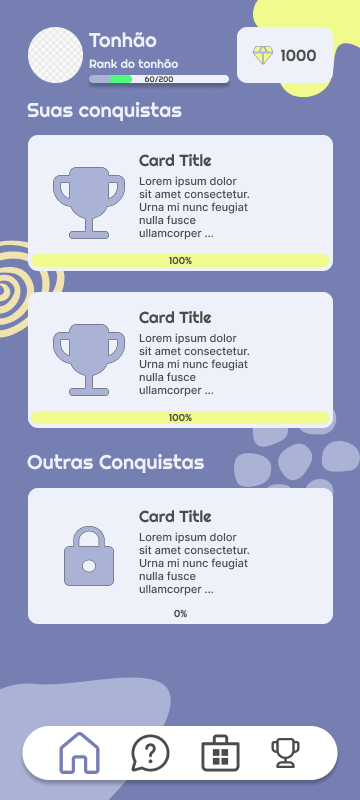
\includegraphics[scale=0.7]{figuras/Math.Pow App/Achievements Alternative BG.png}
    \caption{Prototipação de telas: Autoral desenvolvida pela equipe Tela 01, 2024.}
    \label{fig:nome-da-imagem}
\end{figure}

\begin{figure}
    \centering
    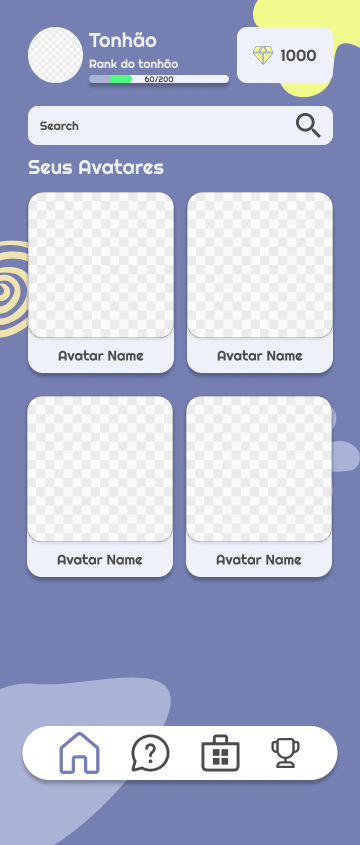
\includegraphics[scale=0.7]{figuras/Math.Pow App/AvatarPage.png}
    \caption{Prototipação de telas: Autoral desenvolvida pela equipe Tela 02, 2024.}
    \label{fig:nome-da-imagem}
\end{figure}

\begin{figure}
    \centering
    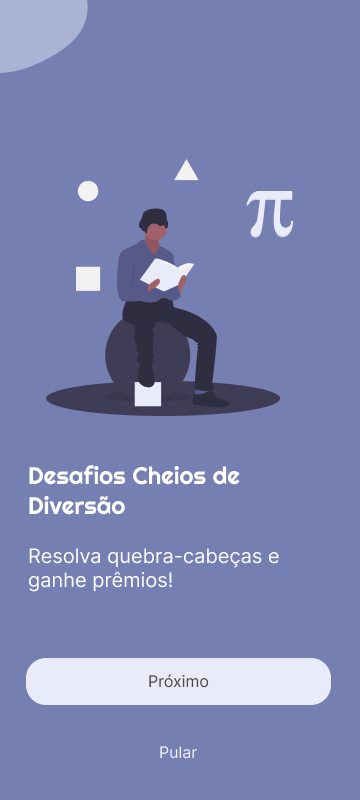
\includegraphics[scale=0.7]{figuras/Math.Pow App/challenges.png}
    \caption{Prototipação de telas: Autoral desenvolvida pela equipe Tela 03, 2024.}
    \label{fig:nome-da-imagem}
\end{figure}

\begin{figure}
    \centering
    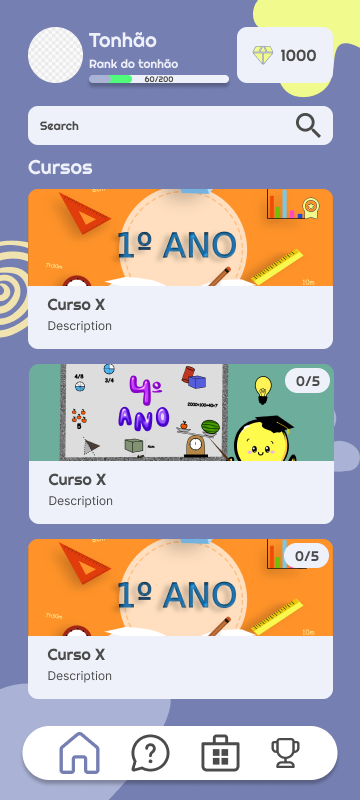
\includegraphics[scale=0.7]{figuras/Math.Pow App/Courses Page.png}
    \caption{Prototipação de telas: Autoral desenvolvida pela equipe Tela 04, 2024.}
    \label{fig:nome-da-imagem}
\end{figure}

\begin{figure}
    \centering
    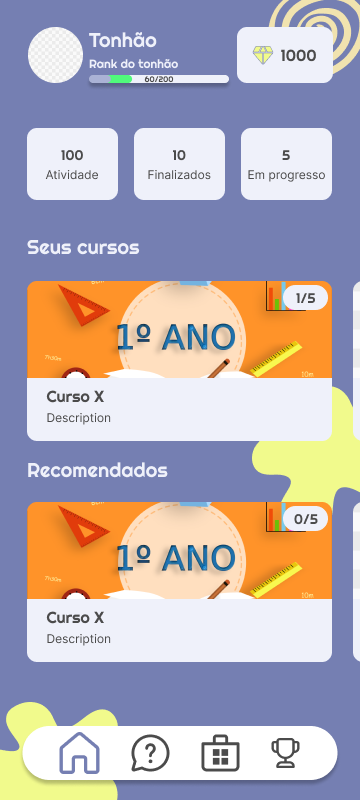
\includegraphics[scale=0.7]{figuras/Math.Pow App/Home Alternative BG.png}
    \caption{Prototipação de telas: Autoral desenvolvida pela equipe Tela 05, 2024.}
    \label{fig:nome-da-imagem}
\end{figure}

\begin{figure}
    \centering
    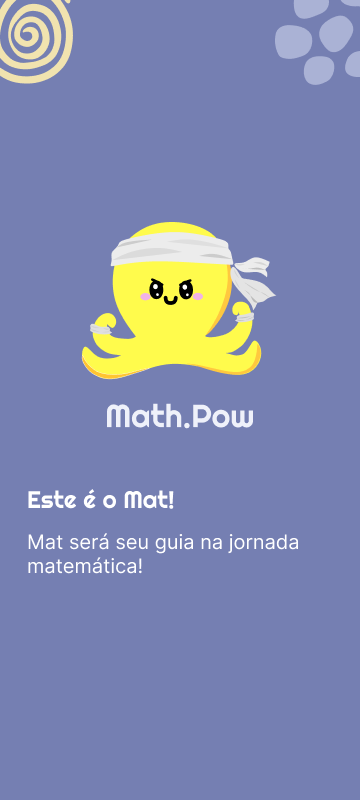
\includegraphics[scale=0.7]{figuras/Math.Pow App/Initial.png}
    \caption{Prototipação de telas: Autoral desenvolvida pela equipe Tela 06, 2024.}
    \label{fig:nome-da-imagem}
\end{figure}

\begin{figure}
    \centering
    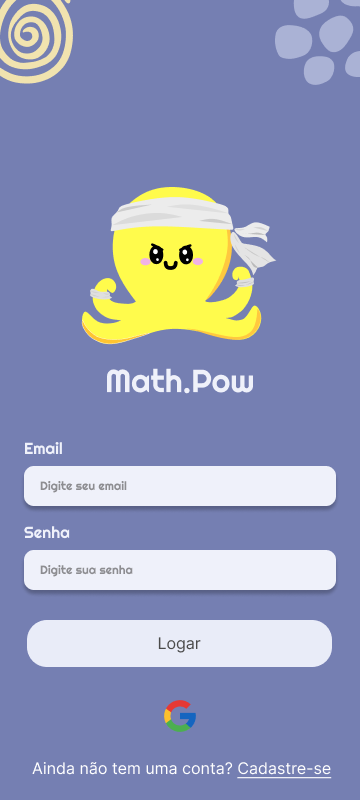
\includegraphics[scale=0.7]{figuras/Math.Pow App/Login.png}
    \caption{Prototipação de telas: Autoral desenvolvida pela equipe Tela 07, 2024.}
    \label{fig:nome-da-imagem}
\end{figure}

\begin{figure}
    \centering
    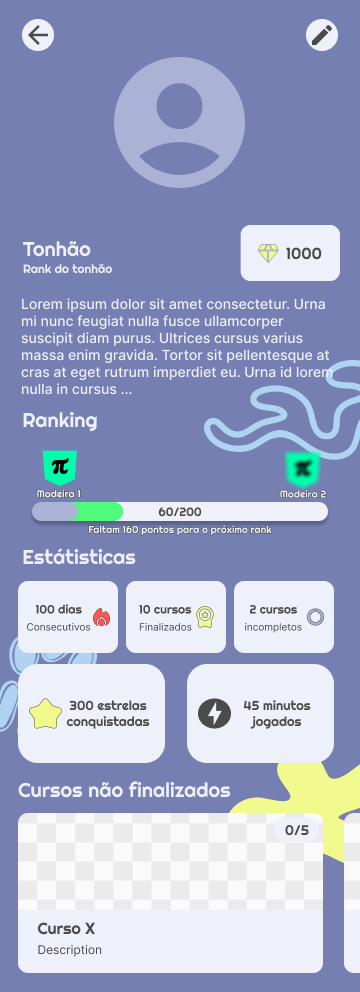
\includegraphics[scale=0.7]{figuras/Math.Pow App/Profile V3.png}
    \caption{Prototipação de telas: Autoral desenvolvida pela equipe Tela 08, 2024.}
    \label{fig:nome-da-imagem}
\end{figure}

\begin{figure}
    \centering
    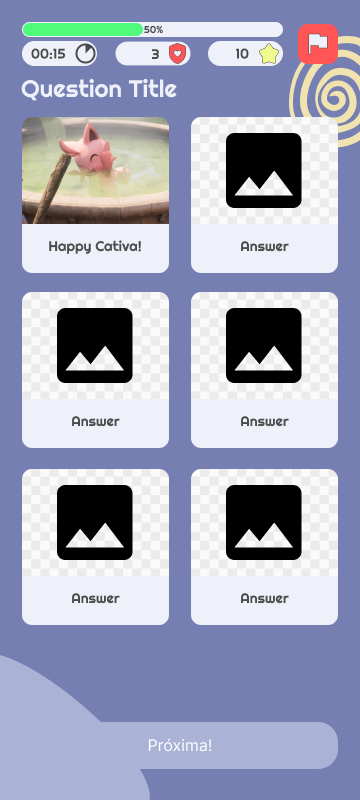
\includegraphics[scale=0.7]{figuras/Math.Pow App/Question Multiple Choice Image Only.png}
    \caption{Prototipação de telas: Autoral desenvolvida pela equipe Tela 09, 2024.}
    \label{fig:nome-da-imagem}
\end{figure}

\begin{figure}
    \centering
    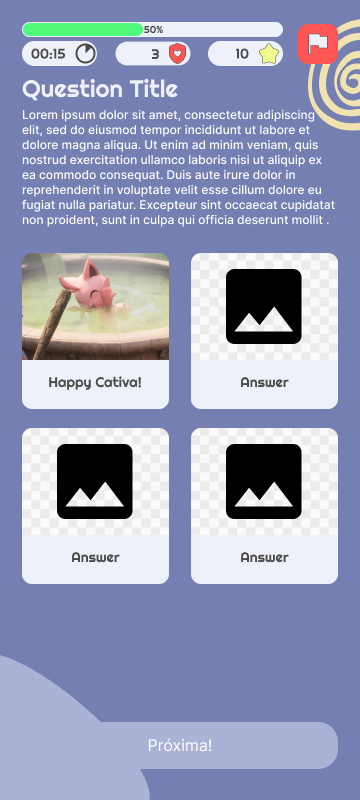
\includegraphics[scale=0.7]{figuras/Math.Pow App/Question Multiple Choice Image With Text.png}
    \caption{Prototipação de telas: Autoral desenvolvida pela equipe Tela 10, 2024.}
    \label{fig:nome-da-imagem}
\end{figure}

\begin{figure}
    \centering
    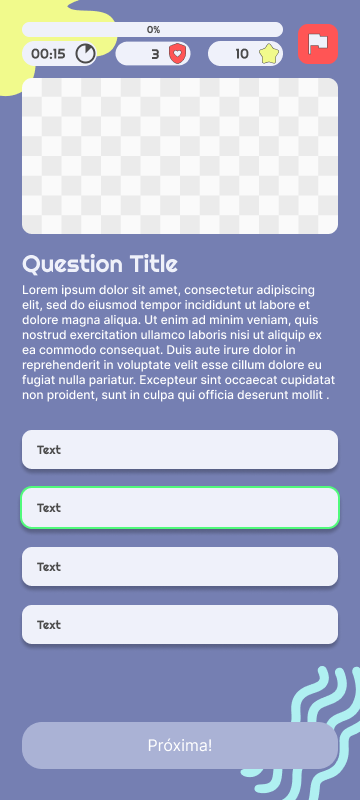
\includegraphics[scale=0.7]{figuras/Math.Pow App/Question Multiple Choice WIth Image.png}
    \caption{Prototipação de telas: Autoral desenvolvida pela equipe Tela 11, 2024.}
    \label{fig:nome-da-imagem}
\end{figure}

\begin{figure}
    \centering
    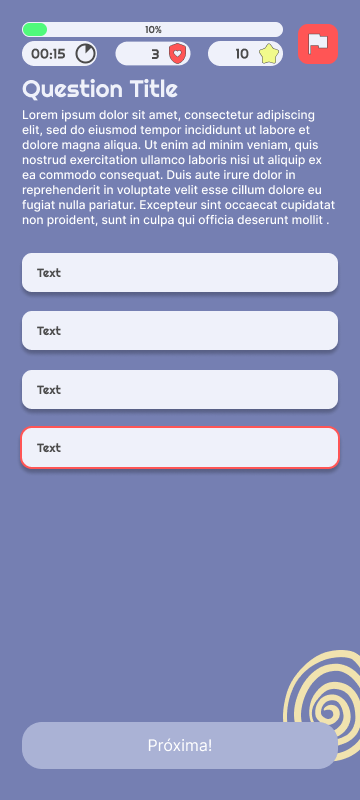
\includegraphics[scale=0.7]{figuras/Math.Pow App/Question Multiple Choice Without Image.png}
    \caption{Prototipação de telas: Autoral desenvolvida pela equipe Tela 12, 2024.}
    \label{fig:nome-da-imagem}
\end{figure}


\begin{figure}
    \centering
    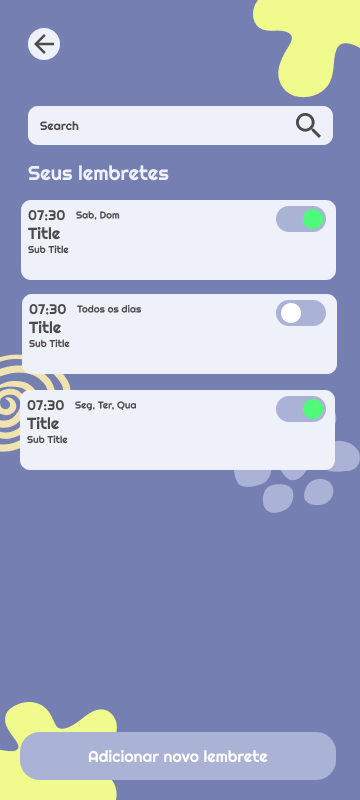
\includegraphics[scale=0.7]{figuras/Math.Pow App/Reminders (1).png}
    \caption{Prototipação de telas: Autoral desenvolvida pela equipe Tela 13, 2024.}
    \label{fig:nome-da-imagem}
\end{figure}

\begin{figure}
    \centering
    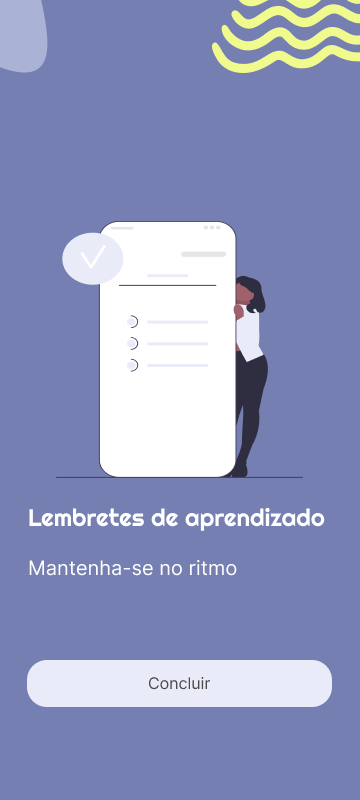
\includegraphics[scale=0.7]{figuras/Math.Pow App/reminders.png}
    \caption{Prototipação de telas: Autoral desenvolvida pela equipe Tela 14, 2024.}
    \label{fig:nome-da-imagem}
\end{figure}

\begin{figure}
    \centering
    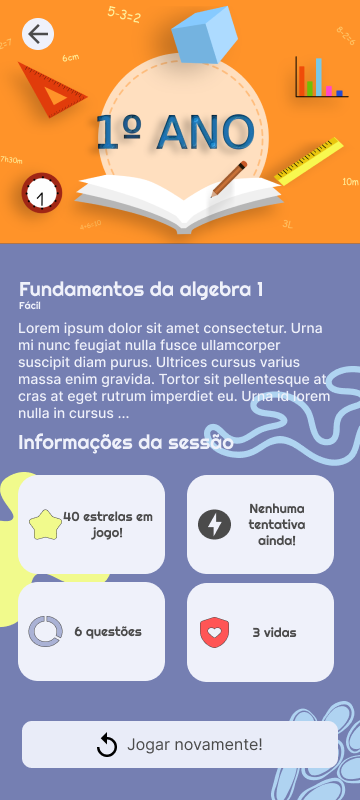
\includegraphics[scale=0.7]{figuras/Math.Pow App/Seassion_Page_V3.png}
    \caption{Prototipação de telas: Autoral desenvolvida pela equipe Tela 15, 2024.}
    \label{fig:nome-da-imagem}
\end{figure}

\begin{figure}
    \centering
    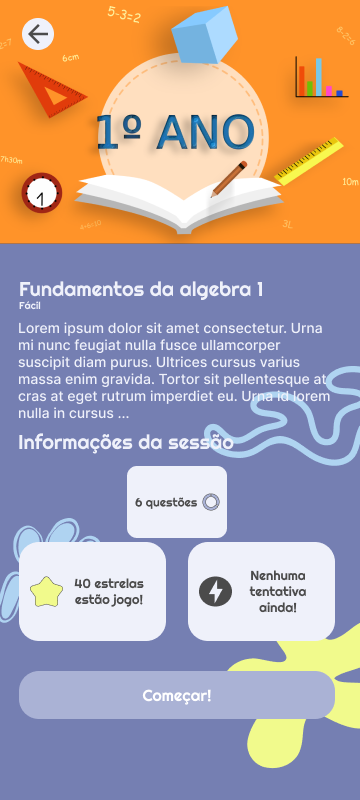
\includegraphics[scale=0.7]{figuras/Math.Pow App/Seassion_Page.png}
    \caption{Prototipação de telas: Autoral desenvolvida pela equipe Tela 16, 2024.}
    \label{fig:nome-da-imagem}
\end{figure}

\begin{figure}
    \centering
    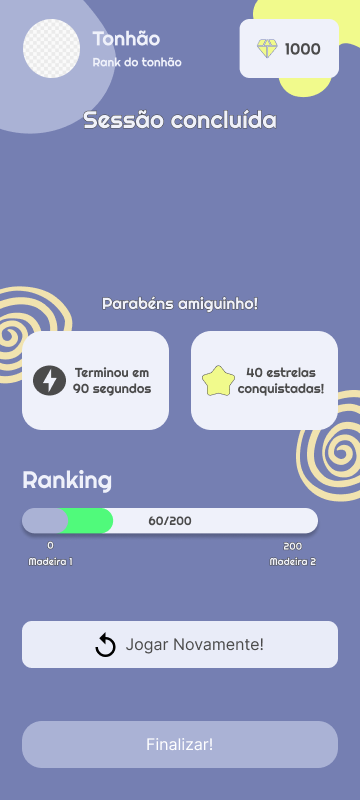
\includegraphics[scale=0.7]{figuras/Math.Pow App/Sesson Ending.png}
    \caption{Prototipação de telas: Autoral desenvolvida pela equipe Tela 17, 2024.}
    \label{fig:nome-da-imagem}
\end{figure}

\begin{figure}
    \centering
    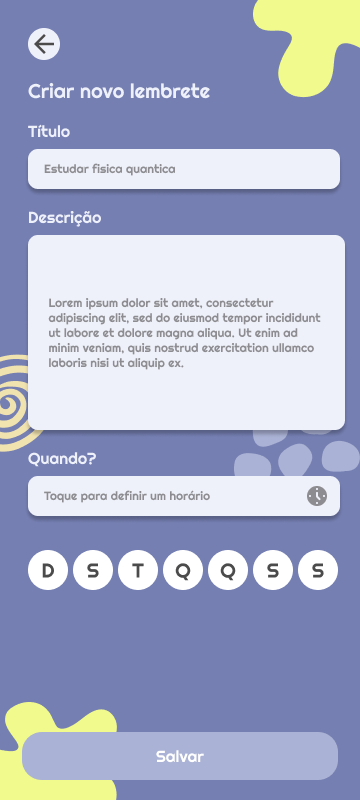
\includegraphics[scale=0.7]{figuras/Math.Pow App/Set a Reminder.png}
    \caption{Prototipação de telas: Autoral desenvolvida pela equipe Tela 18, 2024.}
    \label{fig:nome-da-imagem}
\end{figure}

\begin{figure}
    \centering
    
\includegraphics[scale=0.7]{figuras/Math.Pow App/SplashScreen.png}
    \caption{Prototipação de telas: Autoral desenvolvida pela equipe Tela 19, 2024.}
    \label{fig:nome-da-imagem}
\end{figure}

\begin{figure}
    \centering
    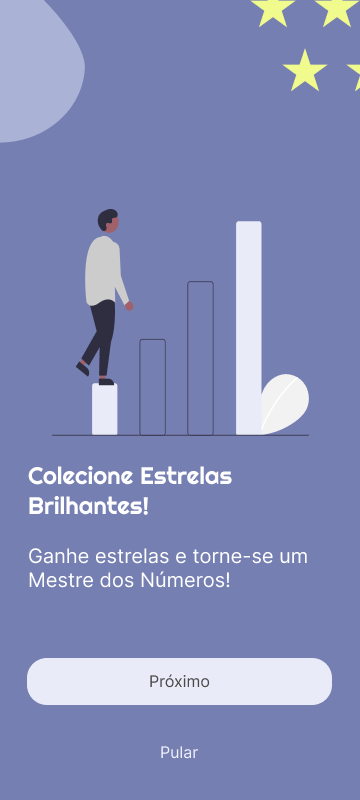
\includegraphics[scale=0.7]{figuras/Math.Pow App/stars.png}
    \caption{Prototipação de telas: Autoral desenvolvida pela equipe Tela 20, 2024.}
    \label{fig:nome-da-imagem}
\end{figure}

\begin{figure}
    \centering
    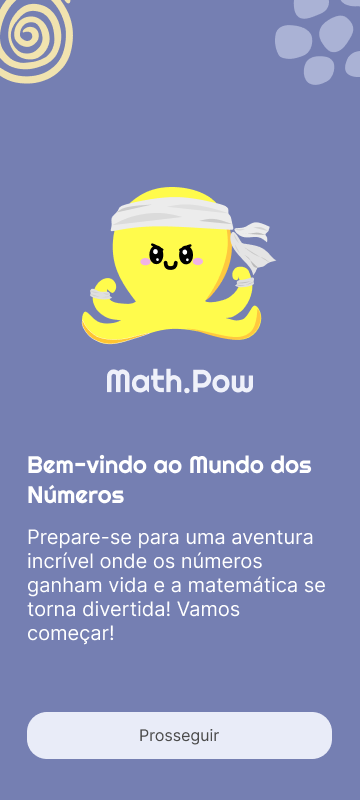
\includegraphics[scale=0.7]{figuras/Math.Pow App/Welcome.png}
    \caption{Prototipação de telas: Autoral desenvolvida pela equipe Tela 21, 2024.}
    \label{fig:nome-da-imagem}
\end{figure}

\begin{figure}
    \centering
    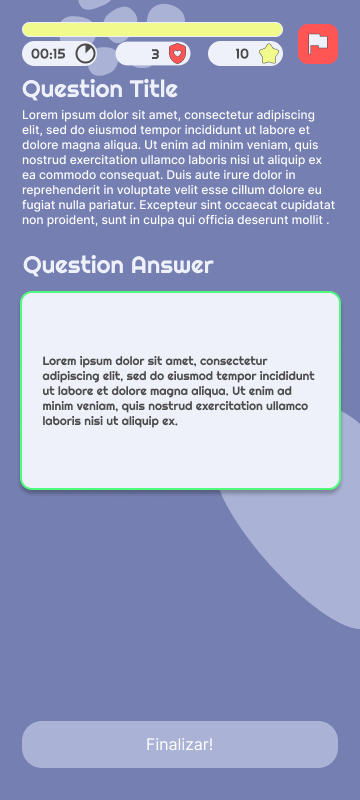
\includegraphics[scale=0.7]{figuras/Math.Pow App/Written Question Without Image.png}
    \caption{Prototipação de telas: Autoral desenvolvida pela equipe Tela 22, 2024.}
    \label{fig:nome-da-imagem}
\end{figure}

\begin{itemize}

    \item \textbf{React Native} 
    \begin{center}
    
\includegraphics[width=0.5\linewidth]{figuras/Tecnologies/React Native.png}
    \captionof{figure}{Logo do framework React Native}
    \label{fig:React Native}
    Fonte para o React Native\footnote{\url{https://reactnative.dev/}}
    \end{center}



    \item \textbf{Docusaurus} 
    \begin{center}
    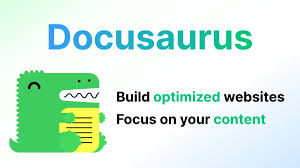
\includegraphics[width=0.5\linewidth]{figuras/Tecnologies/Docusaurus.jpg}
    \captionof{figure}{Logo do framework Docusaurus}
    \label{fig:Docusaurus}
    Fonte para o Docusaurus\footnote{\url{https://docusaurus.io/}}
\end{center}



    
    \item \textbf{Expo}
    \begin{center}
    
\includegraphics[width=0.5\linewidth]{figuras/Tecnologies/Expo Framework.jpeg}
    \captionof{figure}{Logo do framework Expo}
    \label{fig:Expo}
    Fonte para o Expo Framework\footnote{\url{https://expo.dev/}}
\end{center}


    \item \textbf{Firebase}
    \begin{center}
    
\includegraphics[width=0.5\linewidth]{figuras/Tecnologies/Firebase.png}
    \captionof{figure}{Logo do Firebase}
    \label{fig:Firebase}
    Fonte para o Firebase\footnote{\url{https://firebase.google.com/}}
\end{center}




    \item \textbf{TypeScript}
    \begin{center}
    
\includegraphics[width=0.5\linewidth]{figuras/Tecnologies/TypeScript.png}
    \captionof{figure}{Logo do TypeScript}
    \label{fig:TypeScript}
    Fonte para a documentação do TypeScript\footnote{\url{https://www.typescriptlang.org/docs/handbook/typescript-in-5-minutes.html}}
    \end{center}



    \item \textbf{plant UML}
    \begin{center}
    
\includegraphics[width=0.5\linewidth]{figuras/Tecnologies/plantUML.jpeg}
    \captionof{figure}{logo da ferramenta para criação de UMLs PlantUML }
    \label{fig:plant UML}
    Fonte para o plantUML\footnote{\url{https://plantuml.com/}}
    \end{center}




    \item \textbf{Figma}
    \begin{center}
    
\includegraphics[width=0.5\linewidth]{figuras/Tecnologies/Figma.png}
    \captionof{figure}{logo da ferramenta de Design Figma}
    \label{fig:Figma}
    Fonte para o Figma Fonte\footnote{\url{https://www.figma.com/}}
    \end{center}

   
\end{itemize}

\item \textbf{Diagrama de caso de uso}

        \begin{center}
    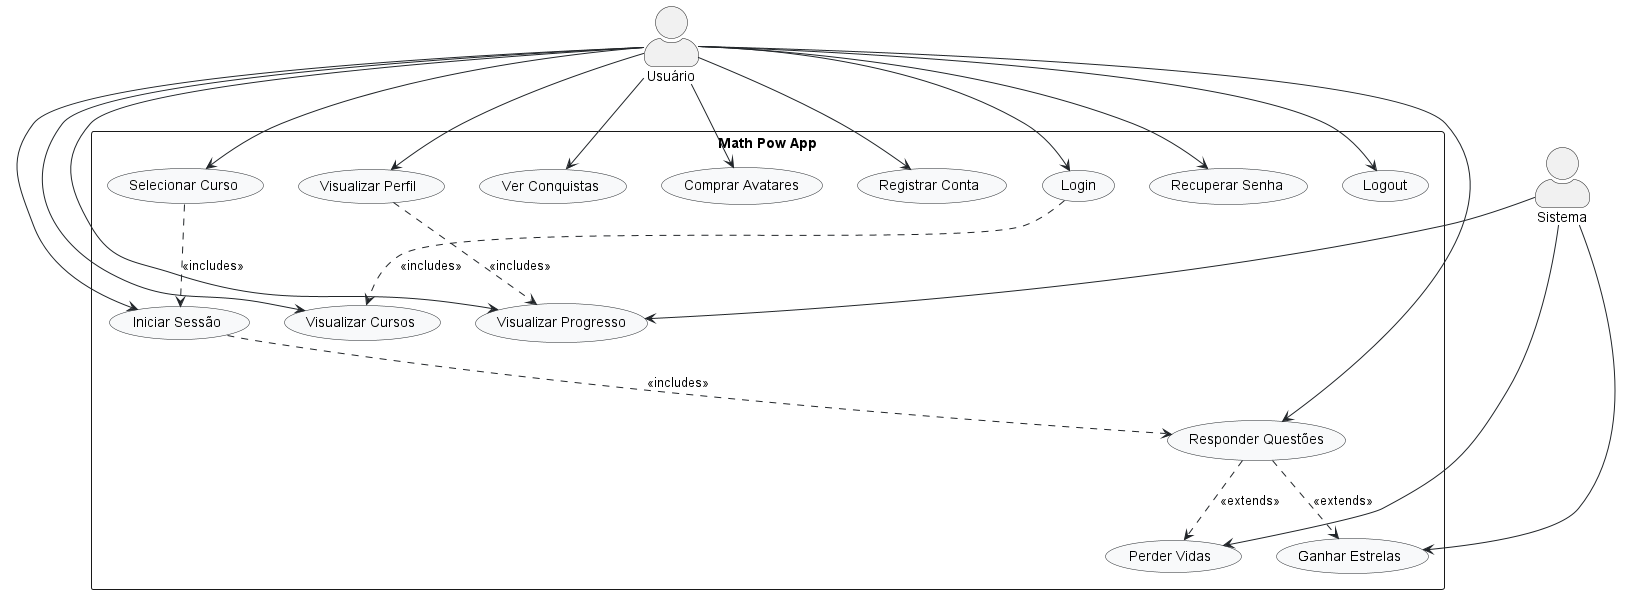
\includegraphics[width=\linewidth]{figuras/DiagramsUMLs/Math Pow Use Case.png}
    \captionof{figure}{Diagrama de caso de uso Fonte: Autoral da equipe}
\end{center}

\end{itemize}

\item \textbf{Diagrama de Classes}

\begin{center}
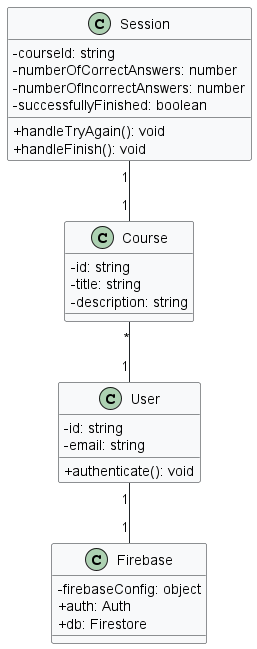
\includegraphics[width=0.3\linewidth]{figuras/DiagramsUMLs/Math Pow App.png}
\captionof{figure}{Diagrama de Classes Fonte: Autoral da equipe}
\label{fig:diagrama-de-classes}
\end{center}

\end{itemize}

\item \textbf{Diagrama de Atividades}

\begin{center}
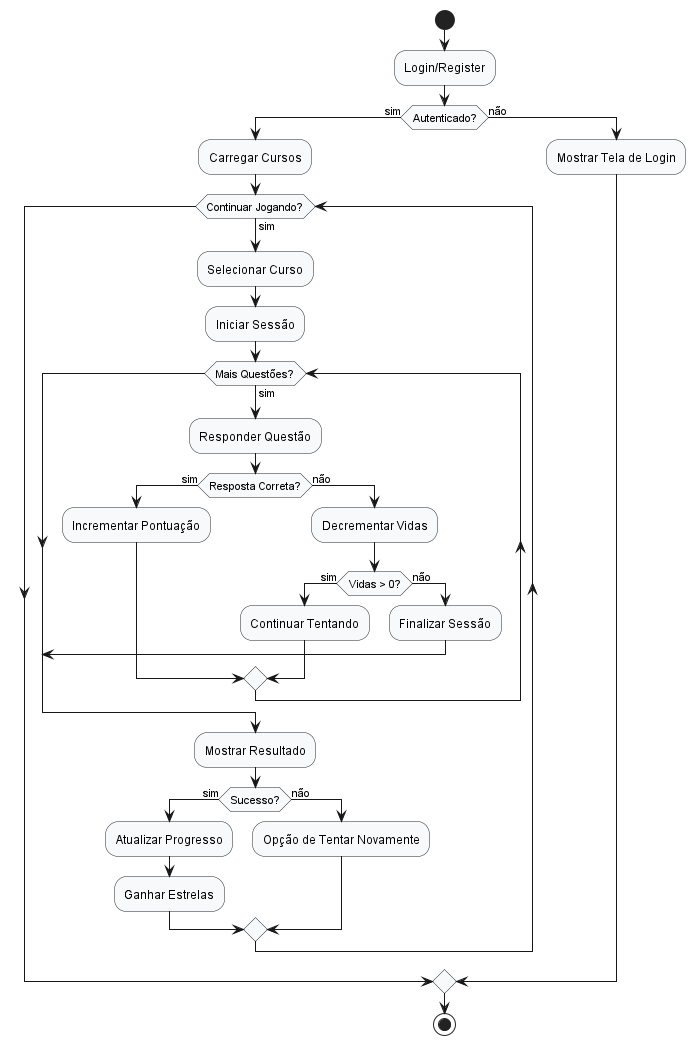
\includegraphics[width=\linewidth]{figuras/DiagramsUMLs/Math Pow Activity.png}
\captionof{figure}{Diagrama de Atividades Fonte: Autoral da equipe}
\label{fig:diagrama-de-atividades}
\end{center}

\end{itemize}

\item \textbf{Diagrama de Sequência}

\begin{center}
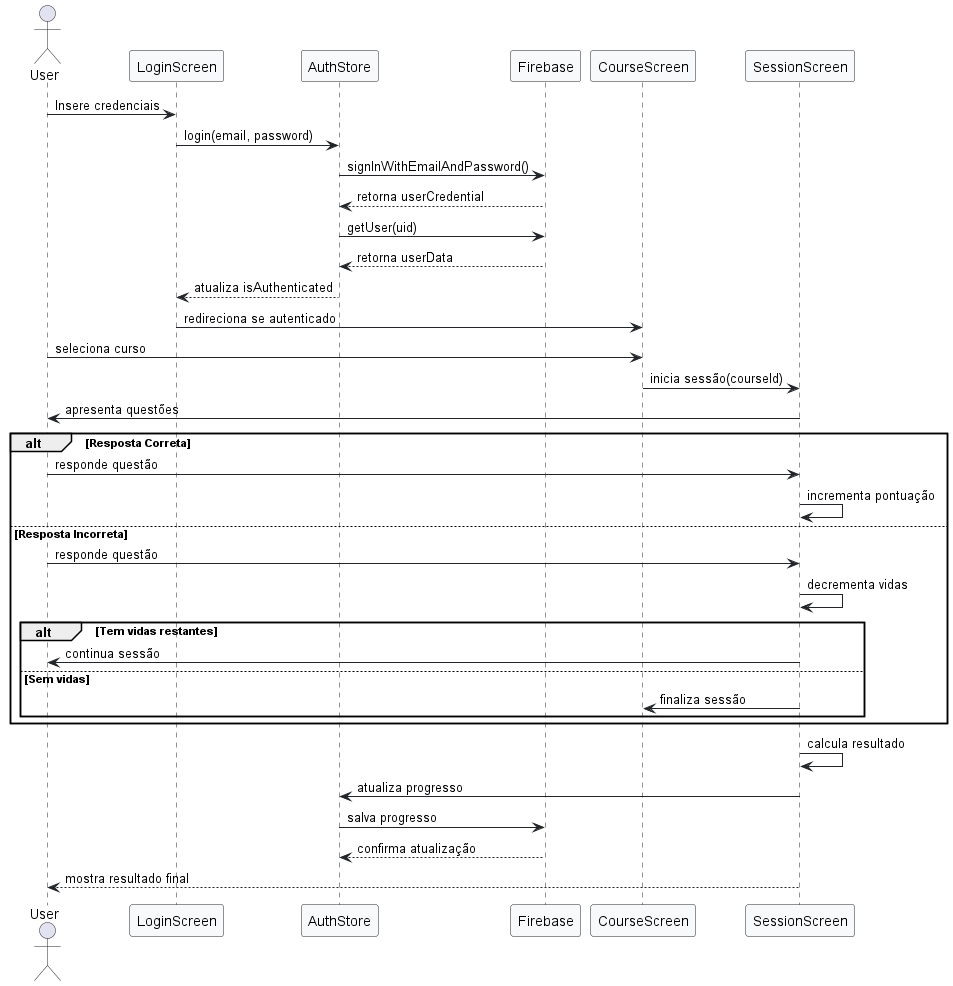
\includegraphics[width=\linewidth]{figuras/DiagramsUMLs/Math Pow Sequence.png}
\captionof{figure}{Diagrama de Sequência Fonte: Autoral da equipe}
\label{fig:diagrama-de-sequencia}
\end{center}

\end{itemize}

\end{document}
